\section{Case analysis}
\label{sec:case}

\subsection{Case settings}
\label{sec:settings}

To verify the effectiveness and applicability of the proposed method, a case study is built entirely from public data.
The deferrable training and batch workload follows the Alibaba PAI GPU cluster trace~\cite{weng2022}, online inference
the Azure LLM inference trace of 2024~\cite{stojkovic2025}, and the weather the ERA5 reanalysis~\cite{hersbach2020} for
Wujiang, Suzhou, retrieved from Open-Meteo; the tariff is the Jiangsu summer TOU tariff of 2025 and the DR rules are
those of Jiangsu~\cite{jiangsu2024dr}. The DR day combines PAI day 27, the weather of 5 August 2024 (maximum
38.3~$^\circ$C) and the Azure trace of 14 May 2024, and the baseline is the mean of the five previous workdays.
\figref{fig:case} shows the inputs: the evening events fall into the TOU peak period after PV output has vanished, and
the grid import without response lies above the baseline during the evening peak because, in normal operation, the
BESS discharges in the peak-price hours that form the baseline.

\begin{figure*}[!t]
\centering
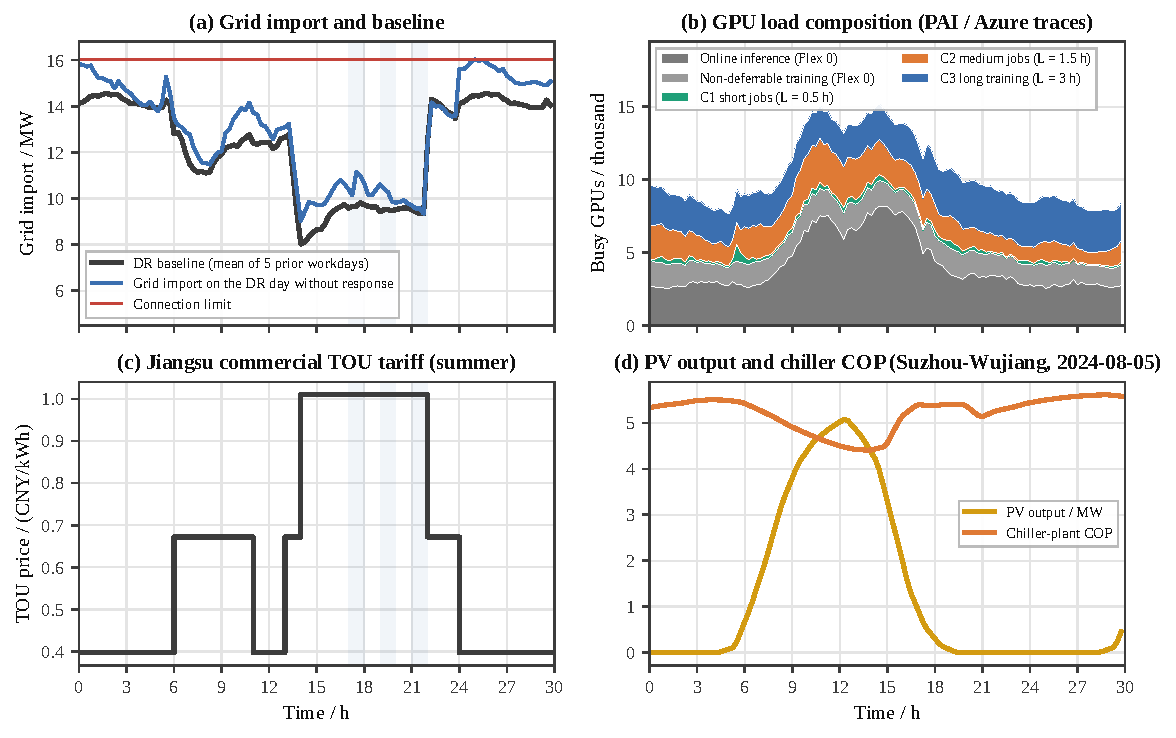
\includegraphics[width=0.86\textwidth]{fig01_case_profiles.pdf}
\caption{Inputs of the case day. (a) DR baseline (mean of the five previous workdays), grid import without response
and connection limit; (b) GPU load composition from the PAI and Azure traces; (c) Jiangsu commercial TOU tariff
(summer); (d) PV output and chiller-plant COP (Wujiang, Suzhou, 5 August 2024). Shaded: the three DR events.}
\label{fig:case}
\end{figure*}

To test the model on LLM-era workloads, the Acme trace of LLM development at the Shanghai AI Laboratory (Seren and
Kalos clusters, March--August 2023)~\cite{hu2024acme} is processed in the same way. It differs strongly from PAI: long
jobs account for 80.5\% of the deferrable GPU$\cdot$h instead of 49.5\%, the GPU$\cdot$h-weighted gang size of the long
class is 407 instead of 35 GPUs, and the load has almost no diurnal cycle (\tabref{tab:acme}). For
\secref{sec:ext-wind}, offshore wind is generated for the Rudong site from ERA5 100-m wind speeds of summer 2024, with a
summer capacity factor of 0.35 and 0.40--0.43 in 17:00--22:00.

Out-of-sample performance is evaluated on 52 operating days: each of the 26 PAI workdays after the DR day is paired with
two different combinations of hot-day weather of summer 2024 and an Azure workday inference trace (a crossed design that
uses no random numbers). The commitments, baseline, scenarios, tuned split $\alpha^*$ and IR-P price are fixed before
the operating day. Statistics are reported as means with 95\% $t$ confidence intervals, and strategies are compared by
paired daily differences with Wilcoxon signed-rank tests. The main parameters are listed in \tabref{tab:params}, with
sources and the parameters of the optional features in \appref{app:data}. Every parameter marked as an assumption is
varied in the sensitivity studies. \tabref{tab:experiments} maps all 26 experiments to the questions they answer.

\begin{table}[!t]
\caption{Main parameters of the case study (sources in \appref{app:data}).}
\label{tab:params}
\centering\footnotesize
\begin{tabularx}{\columnwidth}{@{}>{\raggedright\arraybackslash}p{0.38\columnwidth}X@{}}
\toprule
Parameter & Value\\
\midrule
\multicolumn{2}{@{}l}{\textit{Equipment}}\\
GPUs / node power / idle share & 16,000 / 8.4~kW per 8 GPUs~\cite{latif2024} / 25\%\\
Chiller COP & $6-0.12(T-25)$ in $[3,7]$; 4.41--5.61 on the DR day\\
BESS & 6~MW / 12~MWh, SOC 10--95\%, $\eta=0.95/0.95$, 60~CNY/MWh~\cite{xu2018}\\
TES & 10~MWh$_{\mathrm{th}}$, 4~MW$_{\mathrm{th}}$, $\eta=0.98$, 0.5\%/h\\
Gas engine + absorption & 3~MW, $\eta_{\mathrm e}=0.38$, $\eta_{\mathrm h}=0.45$, 1.5~MW/15~min; COP 0.75\\
PV & 8~MWp, PVWatts v5~\cite{dobos2014}\\
Connection limit $\Pcap=\gamma\hat P$ & $\gamma=1.10\Rightarrow16.03$~MW (1.0--1.3); $P^{\min}=1.5$~MW\\
\multicolumn{2}{@{}l}{\textit{Computing}}\\
Workload & Inference $\approx$25\%, training/batch $\approx$40\% of GPUs, 75\% of it deferrable\\
Lag bounds $L_{1,2,3}$ & 0.5 / 1.5 / 3~h\\
Delay cost / overdue penalty & 0.5 / 1000~CNY per GPU$\cdot$h and hour\\
\multicolumn{2}{@{}l}{\textit{Market and policy}}\\
TOU tariff & Peak 14--22~h ($\times$1.8), valley 0--6~h and 11--13~h ($\times$0.35)\\
DR payment & 3 (E1, E2), 4.2 (E3), 4.8~CNY/kWh (E3 uncertain)\\
Validity / payment cap & $\ge$80\% (+0.1~MW margin) / $\le$120\%\\
Shortfall coefficient $\kappa$ & 1.0 (0.5--2)\\
Rebound charge $\crb$ & 0 and 3~CNY/kW per event (0--6)\\
Gas price & 3.6~CNY/Nm$^3$ (9.89~kWh/Nm$^3$)\\
Emission factors & 0.5617~tCO$_2$/MWh grid~\cite{mee2024ef}; 56.1~t/TJ gas\\
\bottomrule
\end{tabularx}
\end{table}

\begin{table*}[!t]
\caption{Experiments of the case study and where they are reported.}
\label{tab:experiments}
\centering\footnotesize
\setlength{\tabcolsep}{4.5pt}
\begin{tabularx}{\textwidth}{@{}c>{\raggedright\arraybackslash}p{0.21\textwidth}X>{\raggedright\arraybackslash}p{0.14\textwidth}@{}}
\toprule
No. & Experiment & Setting & Reported in\\
\midrule
1 & Cross-event mechanism & Two events; gap $\tau$ 0.25--4~h $\times$ margin $\gamma$ 1.0--1.3; capability ratio & \S\ref{sec:res-mech}, \figref{fig:mech}\\
2 & Case-day closed loop & 8 strategies; coupled and uniform 6-MW commitments; both settlement bases & \S\ref{sec:res-caseday}, \figref{fig:typical}--\ref{fig:flows}\\
3 & Sensitivity (perfect information) & Duration, gap, $\gamma$, commitment; $\tau\times\gamma$ map; hindsight-tuned benchmarks & \S\ref{sec:sens-commit}, \figref{fig:sens}--\ref{fig:map}\\
4 & Out-of-sample evaluation & 52 days; events certain with $\crb=3$ and $\crb=0$; E3 uncertain & \S\ref{sec:res-mc}, \figref{fig:ridge}\\
5 & Channel shadow prices & Duals of the joint plan; KKT residuals & \S\ref{sec:res-price}, \figref{fig:shadow}\\
6 & Commitment--operation pairing & Single-event, scaled single-event and coupled commitments $\times$ IR-O*, JR-D & \S\ref{sec:res-pairing}, \figref{fig:pairing}\\
7 & Ablation and mechanism contribution & No computing flexibility / BESS / TES; waterfall of mechanisms & \S\ref{sec:res-sources}, \figref{fig:decomp}\\
8 & Rebound charge & $\crb$ = 0--6~CNY/kW & \S\ref{sec:sens-rebound}, \figref{fig:rebound}\\
9 & DR payment and shortfall & 1--3~CNY/kWh $\times$ $\kappa$ = 0.5--2 & \S\ref{sec:sens-rebound}, \figref{fig:robust}\\
10 & Realism & Liquid cooling, IT ramp limits, pre-event charge, GPU power capping & \S\ref{sec:sens-real}, \figref{fig:robust}\\
11 & Closed form of Theorem~\ref{thm:closed} & 68 stylised cases, closed form vs LP & \appref{app:proofs}, \figref{fig:theorem}\\
12 & Reliable capacity in closed loop & Uniform 4--9~MW, 20 days & \S\ref{sec:res-capacity}, \figref{fig:capacity}\\
13 & Virtual--physical substitution & BESS 3--24~MWh; $\gamma$ 1.0--1.3; uniform 5--9.5~MW & \S\ref{sec:res-capacity}, \figref{fig:subst}\\
14 & Computational efficiency & Horizon $\times$ scenarios $\times$ events & \S\ref{sec:algorithm}, \tabref{tab:timing}\\
15 & Risk-averse commitment & SP, DRO ($\delta$ = 0.1--1.2), RO, CVaR; 52 days & \S\ref{sec:res-risk}, \figref{fig:risk}\\
16 & Tariff shapes & Five TOU shapes with equal daily mean & \S\ref{sec:sens-gen}, \figref{fig:gen}\\
17 & Multi-energy coupling and policy & Thermal inertia, green share, PUE cap, tie-line ramp & \S\ref{sec:sens-real}, \figref{fig:policy}\\
18 & Season and climate & Suzhou winter, Gui'an summer & \S\ref{sec:sens-gen}, \figref{fig:gen}\\
19 & Job-level validation & PAI/Acme load $\times$ fluid/rigid recovery; 52 days & \S\ref{sec:res-job}, \figref{fig:jobsim}\\
20 & Job mix and overheads & Job sources, gang size $\times$2/$\times$4, checkpoint/restart overheads & \S\ref{sec:res-job}, \figref{fig:jobmix}\\
21 & Green-power direct supply & Offshore wind 0--40~MW behind the meter & \S\ref{sec:ext-wind}, \figref{fig:wind}\\
22 & Pause overhead and capping levels & 6/25-min overheads; one/three capping levels; 26 days & \S\ref{sec:ext-overhead}, \figref{fig:ext}\\
23 & Scenario generation and drift & Quantile vs K-means (+DRO) scenarios; winter day with summer scenarios & \S\ref{sec:res-scen}, \figref{fig:ext}\\
24 & Winter waste-heat recovery & Boiler; heat pump without/with 20 and 40~MWh tanks; 26 winter days & \S\ref{sec:ext-heat}, \figref{fig:heat}\\
25 & Capability region & 91 rays $\times$ 5 strategies; slices; gap $\times$ margin; 52 days & \S\ref{sec:res-region}, \figref{fig:region}\\
26 & Distributed coordination & Plan--price iteration in open loop; JR-A with 1/3/10 exchanges per step; 52 days & \S\ref{sec:res-admm}, \figref{fig:admm}\\
\bottomrule
\end{tabularx}
\end{table*}

\subsection{Cross-event mechanism and closed-loop performance}
\label{sec:res-performance}

\subsubsection{Cross-event recovery mechanism and theoretical checks}
\label{sec:res-mech}

Two events are considered first: a preceding event A from 17:00 and a subsequent event B that starts after a gap
$\tau$. \figref{fig:mech} compares the maximum sustainable reduction $\Gamma_B$ of event B with its stand-alone
capability $\Gamma_B^0$, and \tabref{tab:mech} lists the case with A = 6~MW $\times$ 2~h, B = 1~h and $\gamma=1.10$.
When event A ends, the backlog energy is 4.9~MWh, the storage deficit 12.3~MWh and $\Gamma_B^0\approx8.0$~MW.

\begin{figure*}[!t]
\centering
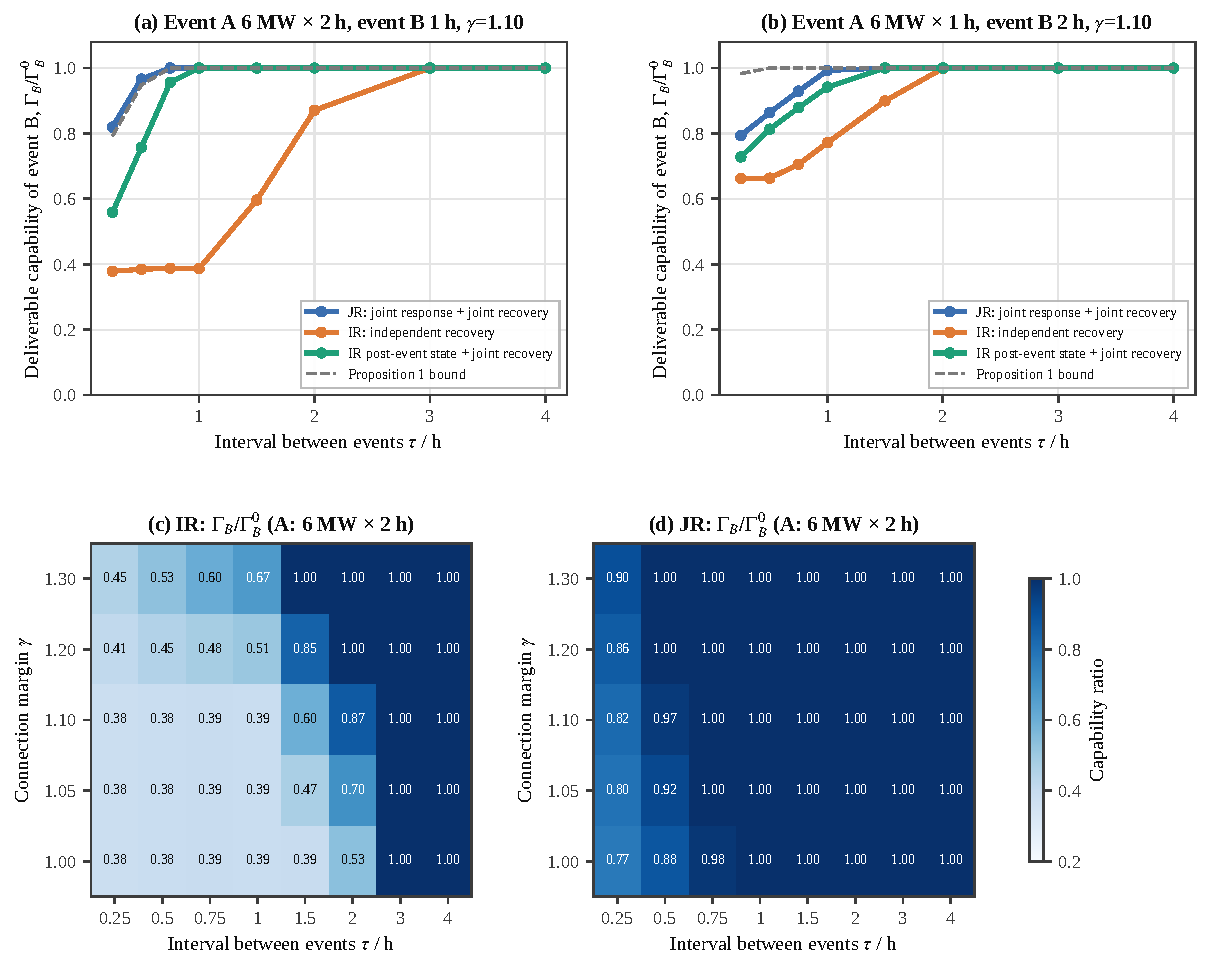
\includegraphics[width=0.84\textwidth]{fig02_mechanism.pdf}
\caption{Cross-event recovery mechanism. (a)(b) Deliverable capability of event B relative to its stand-alone capability
versus the gap ($\gamma=1.10$); (c)(d) capability ratio of independent and joint recovery on the gap--margin plane
(event A: 6~MW $\times$ 2~h).}
\label{fig:mech}
\end{figure*}

\begin{table}[!t]
\caption{Deliverable capability ratio $\Gamma_B/\Gamma_B^0$ (event A 6~MW $\times$ 2~h, event B 1~h, $\gamma=1.10$).}
\label{tab:mech}
\centering\footnotesize
\setlength{\tabcolsep}{3.3pt}
\begin{tabular}{@{}cccccc@{}}
\toprule
Gap $\tau$ (h) & $H$ (MWh) & IR & \makecell{IR state +\\joint recovery} & \makecell{JR (joint response\\and recovery)} & \makecell{Bound of\\Prop.~\ref{prop:bound}}\\
\midrule
0.25 & 1.65 & 0.38 & 0.56 & 0.82 & 0.79\\
0.50 & 3.28 & 0.38 & 0.76 & 0.97 & 0.95\\
0.75 & 4.91 & 0.39 & 0.96 & 1.00 & 1.00\\
1.00 & 6.55 & 0.39 & 1.00 & 1.00 & 1.00\\
1.50 & 9.80 & 0.60 & 1.00 & 1.00 & 1.00\\
2.00 & 13.02 & 0.87 & 1.00 & 1.00 & 1.00\\
\bottomrule
\multicolumn{6}{@{}p{0.97\columnwidth}@{}}{\scriptsize The bound is evaluated at the post-event state of IR, so JR, which also changes the response in event A, may exceed it.}
\end{tabular}
\end{table}

Independent recovery must repay the whole debt before it can respond again: for gaps of up to 1~h, event B retains
only 38--39\% of its stand-alone capability, and 87\% is reached only after 2~h. Joint recovery repays only what the
next event needs. From the same post-event state, a gap of 0.75~h, whose channel energy is only 29\% of the total debt,
already restores 96\%; if the preceding response is planned jointly as well, 0.5~h suffices for 97\%. When event B is
longer (A 1~h, B 2~h), the energy-type limit becomes more prominent: for $\tau\le1$~h, IR reaches 0.66--0.77, joint
recovery from the IR state 0.73--0.94 and JR 0.79--0.99.

The bound of Proposition~\ref{prop:bound} holds in all 80 cases, never exceeding the optimal value from the same
post-event state, and is within 0.05~MW of it in 47 cases; the looser cases occur for $\tau\le0.5$~h, where the
channel width, charging power and EDF order cannot be shifted freely in time while $H$ counts only the total. The
closed form of Theorem~\ref{thm:closed} agrees with the discrete-time LP in all 68 stylised cases to within
$1\times10^{-5}$~MW (\figref{fig:theorem}). With $p_f=5$~MW, $X=5$~MWh and $h=3$~MW, the minimum full-recovery gaps of
IR and JR differ by 0, 0.83, 1.67 and 1.67~h for $L$ = 1, 1.5, 2 and 3~h, exactly $\min(X,p_f(L-D_B))/h$, and joint
recovery has no value when $L=1$~h equals the duration of event B, as predicted by Corollary~\ref{cor:novalue}(a).

\subsubsection{Case-day comparison under identical commitments}
\label{sec:res-caseday}

All strategies are run in closed loop with 15-min steps, the same commitments, SLA and physical constraints, and are
settled by the Jiangsu rules (\tabref{tab:caseday}). Two commitments are used. The coupled day-ahead commitment is
3.27/6.65/7.90~MW for $\crb=3$: because E3 is paid best, the day-ahead model deliberately commits less in E1 and keeps
the channel for E3. For $\crb=0$ it is 8.18/7.98/7.90~MW, equal to the single-event capability assessment. The second
commitment is a uniform 6~MW per event.

\begin{table*}[!t]
\caption{Case-day results: fulfilment / valid events / maximum rebound (MW) / total cost ($10^4$~CNY).}
\label{tab:caseday}
\centering\footnotesize
\setlength{\tabcolsep}{4.2pt}
\begin{tabular}{@{}llllllc@{}}
\toprule
Commitment and settlement & IR-O* & IR-P & JR-M & \textbf{JR-D} & JR-S & JR-oracle\\
\midrule
Coupled, $\crb=3$ & 100\% / 3 / 6.39 / 24.35 & 100\% / 3 / 4.16 / 23.31 & 86.0\% / 2 / 6.44 / 28.01 & \textbf{99.9\% / 3 / 5.02 / 22.71} & 100\% / 3 / 3.48 / 22.76 & 22.66\\
Uniform 6~MW, $\crb=3$ & 100\% / 3 / 6.45 / 24.57 & 96.6\% / 3 / 4.37 / 23.61 & 92.4\% / 2 / 6.44 / 26.42 & \textbf{100\% / 3 / 5.77 / 22.84} & 100\% / 3 / 4.77 / 22.85 & 22.80\\
Coupled, $\crb=0$ & 80.3\% / 2 / -- / 22.70 & 73.7\% / 1 / -- / 24.70 & 84.4\% / 2 / -- / 24.60 & \textbf{99.3\% / 3 / -- / 19.13} & 99.6\% / 3 / -- / 19.12 & 19.04\\
Uniform 6~MW, $\crb=0$ & 100\% / 3 / -- / 19.97 & 92.6\% / 3 / -- / 20.42 & 99.8\% / 3 / -- / 20.81 & \textbf{100\% / 3 / -- / 19.34} & 100\% / 3 / -- / 19.36 & --\\
\bottomrule
\multicolumn{7}{@{}l@{}}{\scriptsize With $\crb=0$ all strategies raise the import to near the connection limit after the events (maximum rebound 6.52~MW), so the rebound is not listed.}
\end{tabular}
\end{table*}

\begin{figure*}[!t]
\centering
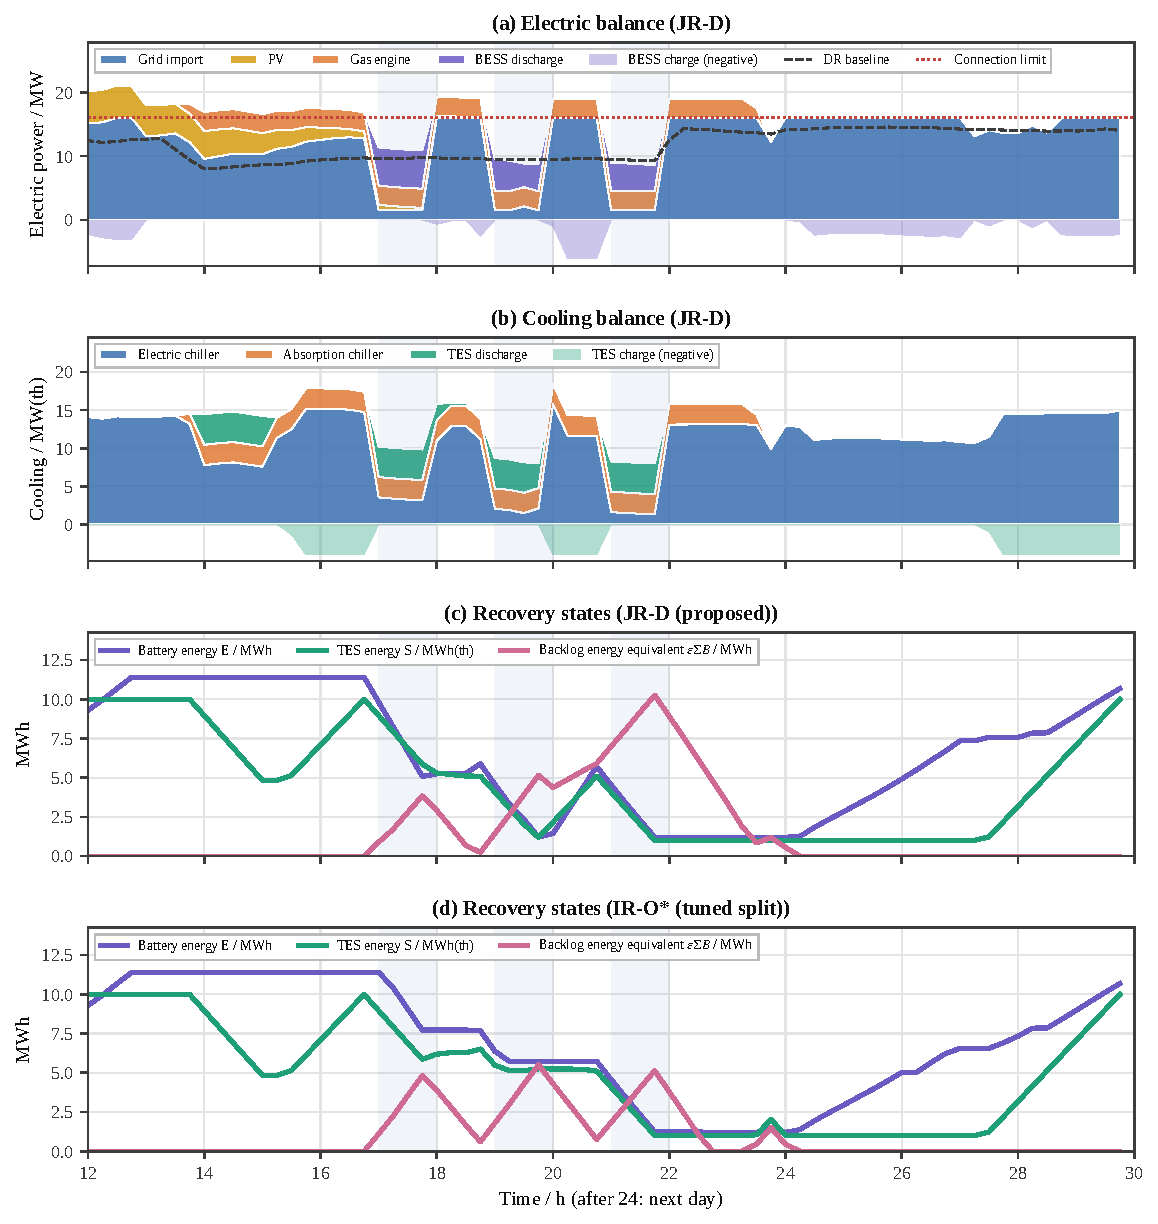
\includegraphics[width=0.80\textwidth]{fig18_typical_day.pdf}
\caption{Operation on the case day (rule setting, coupled commitment 8.18/7.98/7.90~MW). (a) Electricity balance and
(b) cooling balance of JR-D; (c)(d) recovery states of JR-D and IR-O*: BESS energy, TES energy and the electricity
equivalent of the backlog $\varepsilon\sum_cB_c$.}
\label{fig:typical}
\end{figure*}

\begin{figure*}[!t]
\centering
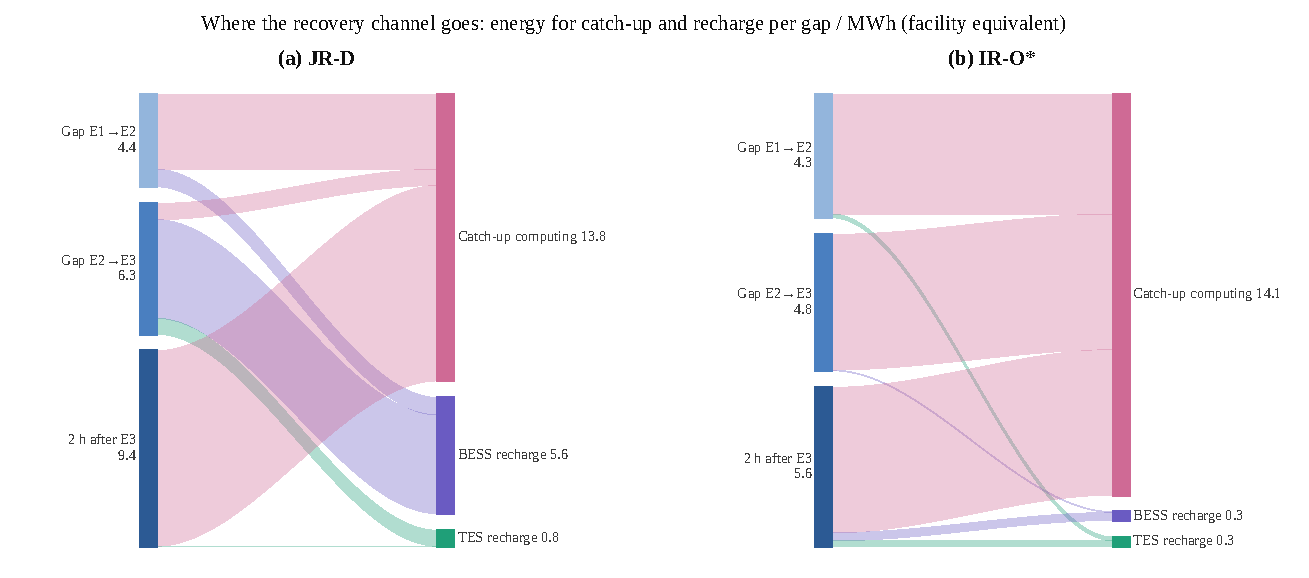
\includegraphics[width=0.78\textwidth]{fig19_channel_flows.pdf}
\caption{Use of the recovery channel in each gap and in the 2~h after E3 (same setting as \figref{fig:typical}):
energy for catch-up computing, BESS recharging and TES recharging.}
\label{fig:flows}
\end{figure*}

Joint recovery is most valuable when the commitments approach the single-event capabilities. In the rule setting with
the coupled commitment, JR-D keeps all three events valid (fulfilment 99.3\%), whereas the strongest independent
benchmark IR-O* fulfils 80.3\% and loses E2; the total cost of JR-D is 15.7\% lower than that of IR-O* and 22.5\% lower
than that of IR-P. \figref{fig:typical} and \figref{fig:flows} show why. JR-D defers more long-lag work during E2, so
that a backlog of 6,027~GPU$\cdot$h, about 10~MWh of facility electricity, is carried into E3; the channel between E2
and E3 is used mainly to recharge the BESS and TES (5.6 and 0.8~MWh), and the backlog is worked off after E3. IR-O*
spends almost the whole channel of the three gaps on catch-up computing (14.1~MWh) and recharges only 0.3~MWh of
storage; in E2 its energy management gives up validity (delivering 4.76~MW) to save the BESS for the better-paid E3,
and IR-P delivers only 3.40~MW in E2.

With moderate commitments (uniform 6~MW), IR-O* and IR-P keep all three events valid as well, and the advantage of JR-D
shrinks to 3.2\% against IR-O* in the rule setting and 3.3\% against IR-P in the rebound-priced setting. In the rebound-priced setting the
advantage comes mainly from the rebound charge: of the $-2.6\%$ and $-3.3\%$ against IR-P, only $+1.1\%$ and $-0.6\%$
remain when the rebound charge is excluded, because the charge makes the channel expensive after each event and joint
recovery moves catch-up to cheaper hours. Price coordination does not replace joint recovery: IR-P is the strongest
benchmark in the rebound-priced setting but the weakest with high commitments in the rule setting (73.7\%), because a
one-shot day-ahead price is no longer correct once the state deviates from the plan and because the non-unique LP
response lets the IT side crowd the channel again (Proposition~\ref{prop:price}). Cross-event foresight is essential:
the event-by-event JR-M fulfils 84--92\% and costs 8--19\% more than JR-D. The scenario MPC and the perfect-information
reference differ from JR-D by less than 0.5\%.

\subsubsection{Out-of-sample performance on 52 operating days}
\label{sec:res-mc}

\tabref{tab:mc} reports the 52 operating days with a uniform commitment of 6~MW for three settings, and
\figref{fig:ridge} shows the full cost distributions (the box plots are given in \figref{fig:mcbox}). The distribution
of JR-D is shifted to the left as a whole and has the shortest right tail.

\begin{table}[!t]
\caption{Out-of-sample results on 52 operating days (uniform 6~MW; means, 95\% CI in brackets).}
\label{tab:mc}
\centering\footnotesize
\setlength{\tabcolsep}{2.6pt}
\begin{tabular}{@{}lcccc@{}}
\toprule
Strategy & \makecell{Fulfilment\\(\%)} & \makecell{All\\valid} & \makecell{Max rebound\\(MW)} & \makecell{Total cost\\($10^4$~CNY)}\\
\midrule
\multicolumn{5}{@{}l}{\textit{Events certain, $\crb=3$~CNY/kW}}\\
IR-R & 71.1 [66.4, 75.7] & 11.5\% & 6.52 & 30.25 [29.18, 31.33]\\
IR-O & 81.6 [76.9, 86.2] & 48.1\% & 6.28 & 26.00 [24.91, 27.09]\\
IR-O* & 97.8 [96.5, 99.1] & 90.4\% & 6.22 & 24.30 [23.45, 25.15]\\
IR-P & 98.3 [96.7, 99.9] & 94.2\% & 5.30 & 23.20 [22.46, 23.94]\\
JR-M & 91.7 [89.6, 93.8] & 48.1\% & 6.35 & 24.81 [23.78, 25.84]\\
\textbf{JR-D} & \textbf{99.9 [99.7, 100]} & \textbf{100\%} & \textbf{4.85} & \textbf{22.53 [21.79, 23.27]}\\
\multicolumn{5}{@{}l}{\textit{Events certain, $\crb=0$ (Jiangsu settlement only)}}\\
IR-O* & 99.2 [98.5, 99.9] & 98.1\% & 6.5 & 19.71 [19.07, 20.35]\\
IR-P & 93.3 [90.7, 96.0] & 86.5\% & 6.5 & 20.21 [19.42, 20.99]\\
JR-M & 94.6 [92.5, 96.6] & 67.3\% & 6.5 & 21.38 [20.39, 22.36]\\
\textbf{JR-D} & \textbf{99.9 [99.7, 100]} & \textbf{100\%} & 6.5 & \textbf{19.10 [18.54, 19.67]}\\
\multicolumn{5}{@{}l}{\textit{E3 called with probability 0.6, confirmed 1~h ahead, $\crb=3$}}\\
IR-O* & 98.2 & 94.2\% & -- & 24.26\\
IR-P & 97.6 & 94.2\% & -- & 23.67\\
JR-M & 94.9 & 67.3\% & -- & 24.10\\
JR-D & 99.98 & 100\% & -- & 22.74\\
JR-S (scenario tree) & 99.7 & 100\% & -- & 22.65\\
JR-oracle & 100.0 & 100\% & -- & 22.27\\
\bottomrule
\end{tabular}
\end{table}

\begin{figure*}[!t]
\centering
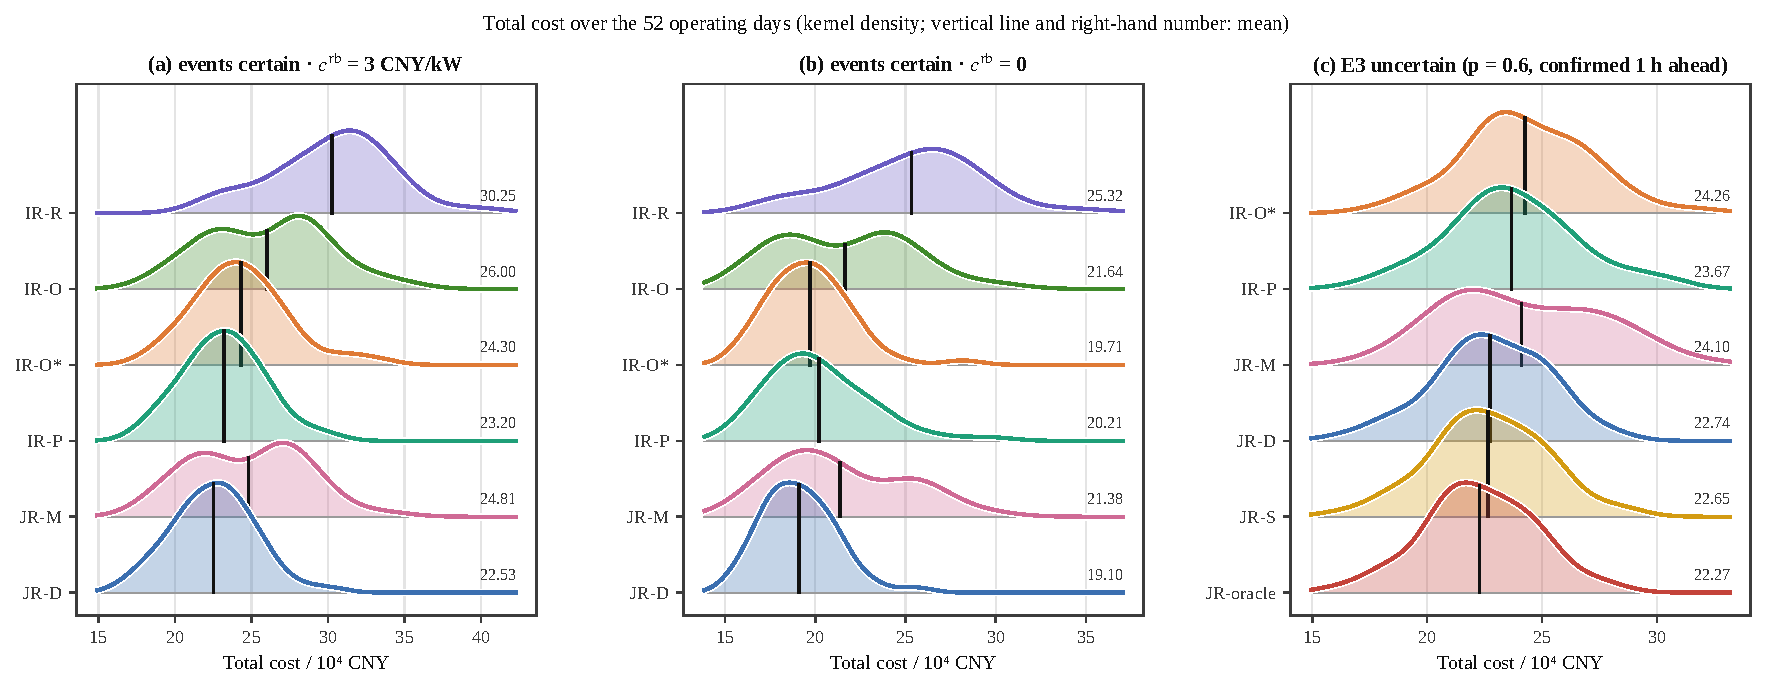
\includegraphics[width=0.94\textwidth]{fig24_ridge_montecarlo.pdf}
\caption{Kernel densities of the daily total cost on the 52 operating days for the three settings (vertical lines and
right-hand numbers: means, $10^4$~CNY).}
\label{fig:ridge}
\end{figure*}

With events certain and the rebound priced, the paired daily difference of JR-D against IR-P is $-6{,}692$~CNY per day
(95\% CI $[-7{,}891,-5{,}492]$, $-2.9\%$, $p=4\times10^{-10}$, cheaper on 50 of the 52 days), with a 8.4\% lower maximum
rebound and 1.6 percentage points higher fulfilment; against IR-O* the cost is 7.3\% lower on all 52 days and the
maximum rebound 22.0\% lower; against JR-M the cost is 9.2\% lower (52/52 days) and the fulfilment 8.2 points higher.
Excluding the rebound charge, the difference to IR-P ($-0.7\%$) is not significant ($p=0.64$), and that to IR-O* is
$+0.9\%$. In the rule setting, JR-D costs 3.1\% less than IR-O* ($-6{,}062$~CNY per day $[-7{,}053,-5{,}072]$, 52/52 days,
$p=4\times10^{-10}$) and 5.5\% less than IR-P; all strategies then raise the import to about 6.5~MW above the baseline
after the events. When E3 is uncertain, JR-D costs 4.0\% less than IR-P (51/52 days) and 6.3\% less than IR-O*. The
scenario MPC gains little: JR-S is 0.4\% cheaper than JR-D ($-821$~CNY per day $[-2{,}064,+421]$, $p=0.46$), saving
5,400~CNY on days when E3 is not called and losing 2,300~CNY on days when it is, so the scenario tree trades part of
the value of called days for a hedge against cancellation. JR-D is 2.1\% above perfect information, mostly because of
the rebound charge (0.2\% without it, $p=0.43$). In summary, against the strongest benchmark of each setting, joint
recovery is 2.9--4.0\% cheaper and keeps all events valid on every day, whereas the benchmarks achieve this on 86--98\%
of the days.

\subsubsection{Sources of benefit and contribution of the mechanisms}
\label{sec:res-sources}

\tabref{tab:ablation} isolates the resources (uniform 6~MW, $\crb=3$, perfect information). Without computing
flexibility ($L=0$) the two strategies are identical: with a single recovery state there is nothing to coordinate. Even
with the hindsight-optimal static split ($\alpha^*=0.9$, fulfilment 100\%), joint recovery is still 6.9\% cheaper.

\begin{table}[!t]
\caption{Ablation (uniform 6~MW, $\crb=3$, perfect information; fulfilment / total cost in $10^4$~CNY).}
\label{tab:ablation}
\centering\footnotesize
\begin{tabular}{@{}lccc@{}}
\toprule
Configuration & IR-O & JR & JR vs IR-O\\
\midrule
Full system & 89.2\% / 25.58 & 100\% / 22.80 & $-10.9\%$\\
No computing flexibility ($L=0$) & 29.0\% / 28.72 & 29.0\% / 28.72 & 0\\
No BESS & 16.4\% / 35.54 & 36.1\% / 32.38 & $-8.9\%$\\
No TES & 68.1\% / 27.03 & 100\% / 23.49 & $-13.1\%$\\
IR-O with hindsight split $\alpha^*=0.9$ & 100\% / 24.49 & -- & $-6.9\%$\\
\bottomrule
\end{tabular}
\end{table}

\begin{figure*}[!t]
\centering
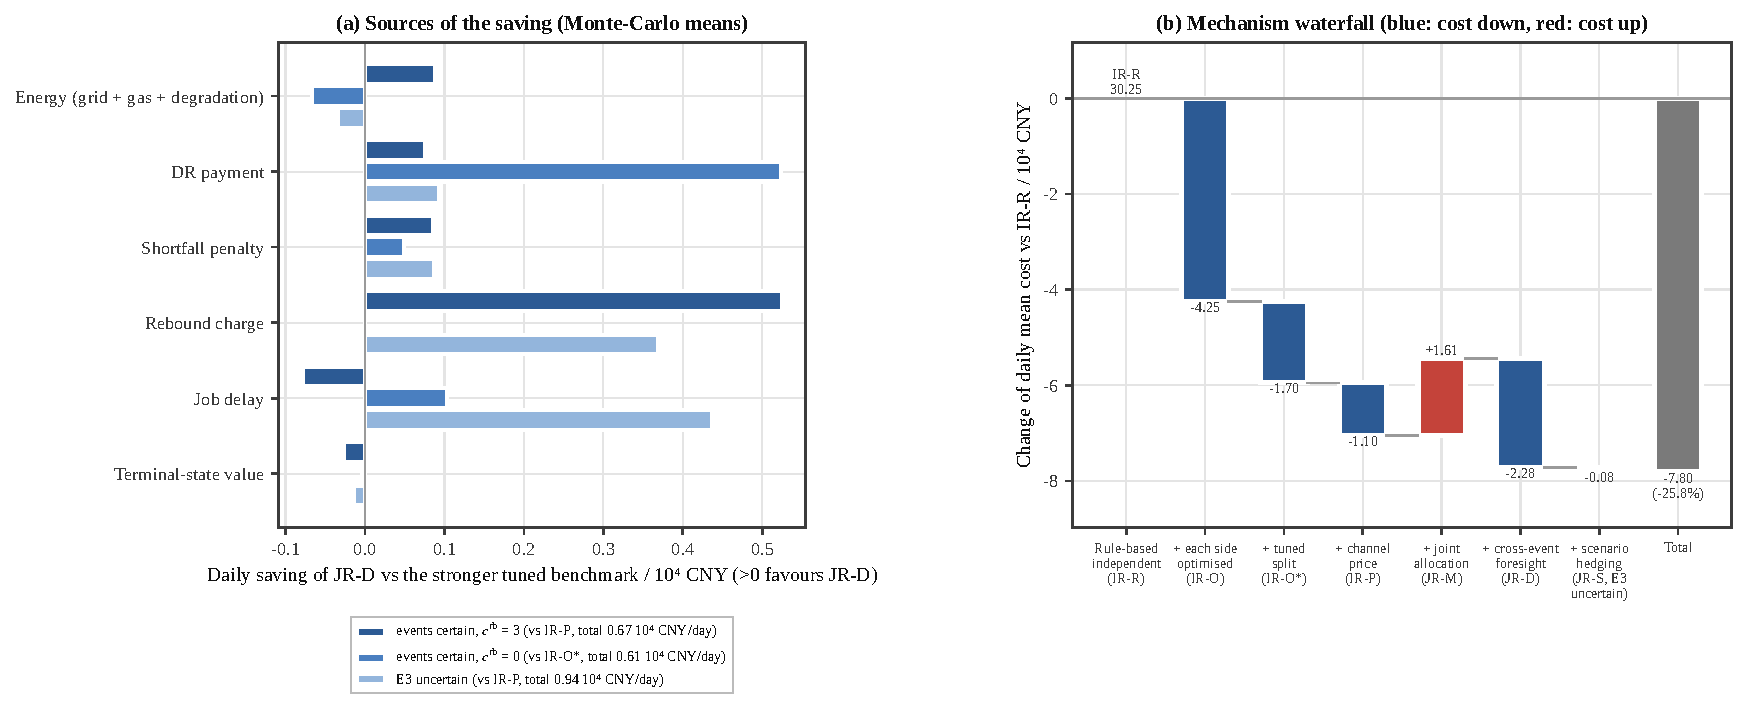
\includegraphics[width=0.94\textwidth]{fig16_decomposition.pdf}
\caption{(a) Daily saving of JR-D against the stronger tuned benchmark, decomposed by source (means over the 52 days);
(b) contribution of each coordination mechanism, starting from rule-based independent recovery (events certain,
$\crb=3$; the last step uses the uncertain-E3 setting).}
\label{fig:decomp}
\end{figure*}

\figref{fig:decomp}(b) adds one coordination mechanism at a time to the rule-based IR-R (30.25$\times10^4$~CNY per day):
optimising each side ($-4.25$), tuning the split on history ($-1.70$), sending the channel price ($-1.10$), allocating
the channel jointly but event by event ($+1.61$), adding cross-event foresight ($-2.28$) and hedging the uncertain event
by scenarios ($-0.08$), a total of $-7.80\times10^4$~CNY ($-25.8\%$). Optimising each side and cross-event foresight
contribute most. Joint allocation without foresight (JR-M) is worse than price coordination, because after each event it
catches up or recharges as if only one more event followed and often spends the channel on the wrong state; joint
allocation and cross-event foresight are both needed.

\figref{fig:decomp}(a) decomposes the daily saving of JR-D against the stronger benchmark. With the rebound priced, 78\%
of the saving of $0.67\times10^4$~CNY against IR-P comes from the rebound charge. In the rule setting, 86\% of the
saving of $0.61\times10^4$~CNY against IR-O* comes from the additional DR payment of keeping all three events valid.
When E3 is uncertain, the largest item is the job-delay cost ($0.44$ of $0.94\times10^4$~CNY), because the IT side of
IR-P follows the day-ahead price and defers too much while the call of E3 is unknown. The energy cost hardly changes in
any setting: joint recovery does not save money by more arbitrage.

\subsection{Deliverable capacity, channel price and coordination}
\label{sec:res-capacity-all}

\subsubsection{Reliably deliverable capacity and virtual--physical substitution}
\label{sec:res-capacity}

In the rule setting, each uniform commitment from 4 to 9~MW was run on 20 operating days in closed loop
(\tabref{tab:capacity}, \figref{fig:capacity}). Requiring all three events to be valid on at least 95\% of the days,
IR-O* can commit 6~MW, IR-P reaches this reliability at no commitment level, and JR-D can commit 8~MW, which is 33\%
more. At the respective best commitments, JR-D (7~MW, $18.89\times10^4$~CNY per day) is 4.1\% cheaper than IR-O* (6~MW,
$19.70\times10^4$~CNY per day).

\begin{table}[!t]
\caption{Closed-loop reliability by uniform commitment (rule setting, 20 days): share of days with all events valid /
mean total cost ($10^4$~CNY).}
\label{tab:capacity}
\centering\footnotesize
\begin{tabular}{@{}cccc@{}}
\toprule
Commitment (MW) & IR-O* & IR-P & \textbf{JR-D}\\
\midrule
4 & 75\% / 21.63 & 85\% / 21.42 & \textbf{100\% / 20.69}\\
5 & 80\% / 20.83 & 75\% / 21.05 & \textbf{100\% / 19.75}\\
6 & 95\% / 19.70 & 80\% / 20.27 & \textbf{100\% / 19.05}\\
7 & 80\% / 20.32 & 70\% / 20.34 & \textbf{95\% / 18.89}\\
8 & 50\% / 21.38 & 40\% / 21.65 & \textbf{95\% / 19.20}\\
9 & 25\% / 22.97 & 25\% / 23.42 & 65\% / 21.01\\
\bottomrule
\end{tabular}
\end{table}

\begin{figure*}[!t]
\centering
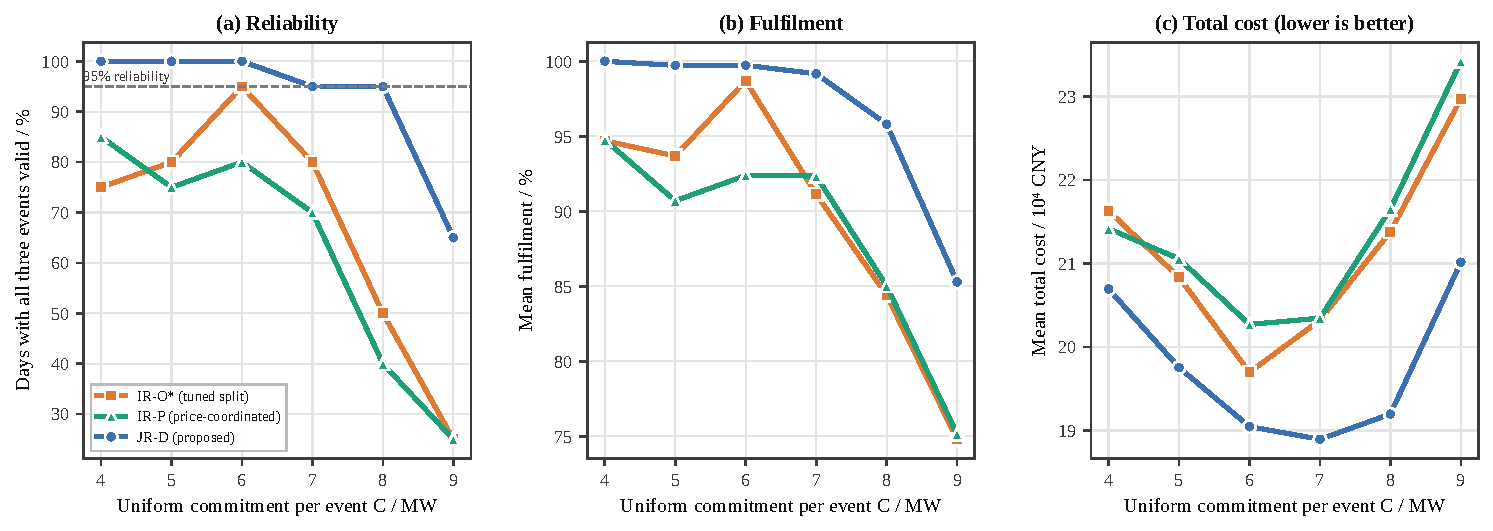
\includegraphics[width=0.94\textwidth]{fig11_capacity.pdf}
\caption{Closed-loop reliability, fulfilment and total cost versus the uniform commitment (rule setting, 20 operating
days).}
\label{fig:capacity}
\end{figure*}

The virtual--physical substitution experiment sweeps the BESS energy (at 6~MW power and a fixed absolute connection
limit) and the connection margin $\gamma$ under perfect information and finds the largest uniform commitment that is
fulfilled at $\ge$99\% with all events valid (\tabref{tab:subst}, \figref{fig:subst}). Joint recovery is worth about
9--12~MWh of battery: JR reaches 6.5~MW with a 3-MWh battery, which IR-O* needs 12~MWh for; JR reaches 7.0~MW with
6~MWh, which IR-O* needs 15--18~MWh for; and JR reaches 8.0~MW with 12~MWh, which independent recovery does not reach
with any battery size. Joint recovery is also worth about 2.9~MW of connection capacity: JR reaches 8.0~MW at
$\gamma=1.10$, whereas IR-O* needs $\gamma=1.30$, \ie\ $0.2\times14.57\approx2.9$~MW more; the 7.0~MW of JR at
$\gamma=1.00$ likewise requires $\gamma=1.20$ for IR-O*. At its reliable capacity, JR carries a long-lag backlog worth
6.0--7.0~MWh into E3, about half of the 12-MWh battery (\figref{fig:subst}(c)); the smaller the battery, the more this
virtual computing storage is used, and with 18~MWh or more the physical storage suffices and joint recovery no longer
needs it.

\begin{table}[!t]
\caption{Reliable uniform commitment (MW, $\ge$99\% fulfilment with all events valid, perfect information).}
\label{tab:subst}
\centering\footnotesize
\setlength{\tabcolsep}{3.6pt}
\begin{tabular}{@{}lccccccc@{}}
\toprule
BESS energy (MWh) & 3 & 6 & 9 & 12 & 15 & 18 & 24\\
\midrule
JR & 6.5 & 7.0 & 7.5 & \textbf{8.0} & 7.5 & 7.0 & 6.5\\
IR-O* (hindsight) & -- & 5.0 & 6.0 & 6.5 & 7.0 & 7.0 & 6.5\\
IR-P & -- & 5.0 & 5.5 & 6.0 & 5.0 & -- & --\\
Backlog carried into E3 by JR (MWh) & 6.8 & 7.0 & 7.0 & 6.0 & 3.5 & 0.8 & 0\\
\midrule
Connection margin $\gamma$ & 1.00 & 1.05 & 1.10 & 1.15 & 1.20 & 1.30 & \\
\midrule
JR & 7.0 & 7.5 & \textbf{8.0} & 8.0 & 8.0 & 8.0 & \\
IR-O* (hindsight) & 6.0 & 6.0 & 6.5 & 6.5 & 7.0 & 8.0 & \\
IR-P & 5.0 & 5.5 & 6.0 & 7.0 & 6.0 & 6.0 & \\
\bottomrule
\multicolumn{8}{@{}l@{}}{\scriptsize --: not reached within the sweep (5--9.5~MW).}
\end{tabular}
\end{table}

\begin{figure*}[!t]
\centering
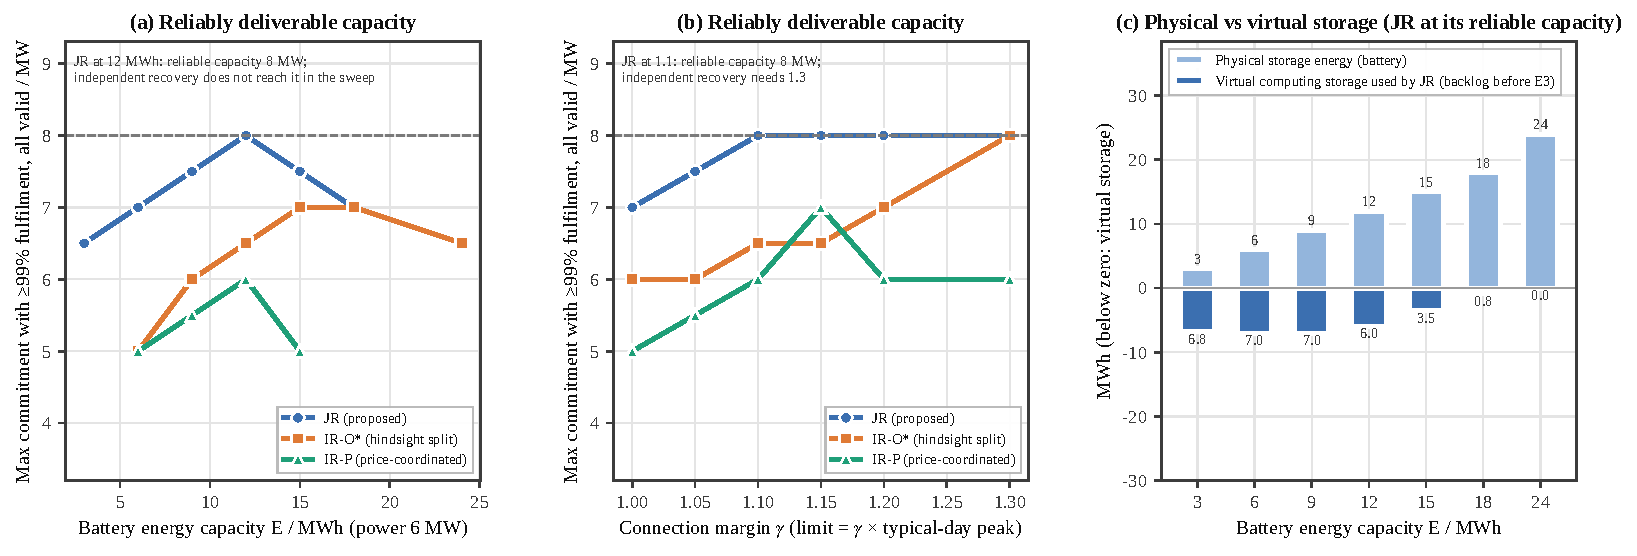
\includegraphics[width=0.96\textwidth]{fig14_substitution.pdf}
\caption{Virtual--physical substitution. (a)(b) Reliably deliverable capacity versus BESS energy and connection margin
(dashed: JR in the base configuration); (c) physical battery energy and the virtual computing storage used by JR
(backlog energy carried into E3) at its reliable capacity.}
\label{fig:subst}
\end{figure*}

Larger batteries are not always better. Beyond 12--15~MWh the reliable capacity of all strategies falls, because in
normal operation a larger battery discharges in the peak-price hours for arbitrage and thereby lowers the
five-day-average baseline: every additional 6~MWh lowers the baseline in the event hours by about 0.6~MW (E1:
10.28~MW with 6~MWh, 8.47~MW with 24~MWh), shrinking the room for reductions measured against it. DR contracts should
therefore consider battery sizing and baseline rules together.

\subsubsection{Shadow prices: scarcity of the recovery channel}
\label{sec:res-price}

With perfect information and a uniform 6~MW, the duals of the joint plan (binaries fixed) reveal the scarcity of the
channel (\tabref{tab:shadow}, \figref{fig:shadow}). Without a rebound charge, the physical connection limit itself
creates competition in the gaps: at $\gamma=1.10$ its shadow price is 1,260--1,455~CNY/MWh (1,771--2,242 at
$\gamma=1.00$), so the channel price is 2.2--3.2 times the peak tariff. With the rebound charge, the binding constraint
becomes the rebound window (3,000~CNY/MWh) and the connection limit is slack. Proposition~\ref{prop:price} is confirmed
numerically: at all interior charging, discharging and catch-up steps of the four settings, the residuals of
$\eta_{\mathrm{c}}\nu_t=\lambda_t+\cdeg$, $\nu_t/\eta_{\mathrm{d}}=\lambda_t-\cdeg$ and $\mu_{c,t}=\varepsilon_t\lambda_t$
are at most $2\times10^{-12}$; for example, $\mu=3.94$~CNY per GPU$\cdot$h in the first gap divided by
$\varepsilon\approx0.99$~kWh per GPU$\cdot$h equals the channel price of about $4.0\times10^3$~CNY/MWh. Long-lag backlog
is the cheapest state: in E3 the marginal cost of C3 backlog (3.19) is well below that of C1 (4.38) because its
deadline lies after E3, so the channel goes first to storage recharging and short-lag catch-up and the long-lag work is
carried across the event, as Theorem~\ref{thm:closed} predicts for several classes.

\begin{table}[!t]
\caption{Shadow prices of the joint plan (CNY/MWh; marginal backlog cost $\mu$ in CNY per GPU$\cdot$h).}
\label{tab:shadow}
\centering\footnotesize
\setlength{\tabcolsep}{3.2pt}
\begin{tabular}{@{}lccccc@{}}
\toprule
Period & $\lambda_t$ & $\lambda^{\mathrm{cap}}_t$ & $\lambda^{\mathrm{rb}}_t$ & $\nu_t$ & $\mu_{1}$ / $\mu_{2}$ / $\mu_{3}$\\
\midrule
\multicolumn{6}{@{}l}{\textit{$\gamma=1.10$, $\crb=3$~CNY/kW}}\\
Gap E1--E2 & 4010 & 0 & 3000 & 4223 & 3.94 / 3.94 / 3.94\\
Gap E2--E3 & 4010 & 0 & 3000 & 4223 & 3.92 / 3.88 / 3.69\\
Event E3 & 4505 & 0 & 0 & 4223 & 4.38 / 3.43 / \textbf{3.19}\\
\multicolumn{6}{@{}l}{\textit{$\gamma=1.10$, $\crb=0$}}\\
Gap E1--E2 & 2464 & \textbf{1455} & 0 & 2657 & 2.49 (all classes)\\
Gap E2--E3 & 2270 & \textbf{1260} & 0 & 2522 & 2.22 (all classes)\\
\multicolumn{6}{@{}l}{\textit{$\gamma=1.00$, $\crb=0$}}\\
Gap E1--E2 & 3252 & \textbf{2242} & 0 & 3285 & 3.16 (all classes)\\
Gap E2--E3 & 2781 & \textbf{1771} & 0 & 3060 & 2.72 (all classes)\\
\bottomrule
\end{tabular}
\end{table}

\begin{figure*}[!t]
\centering
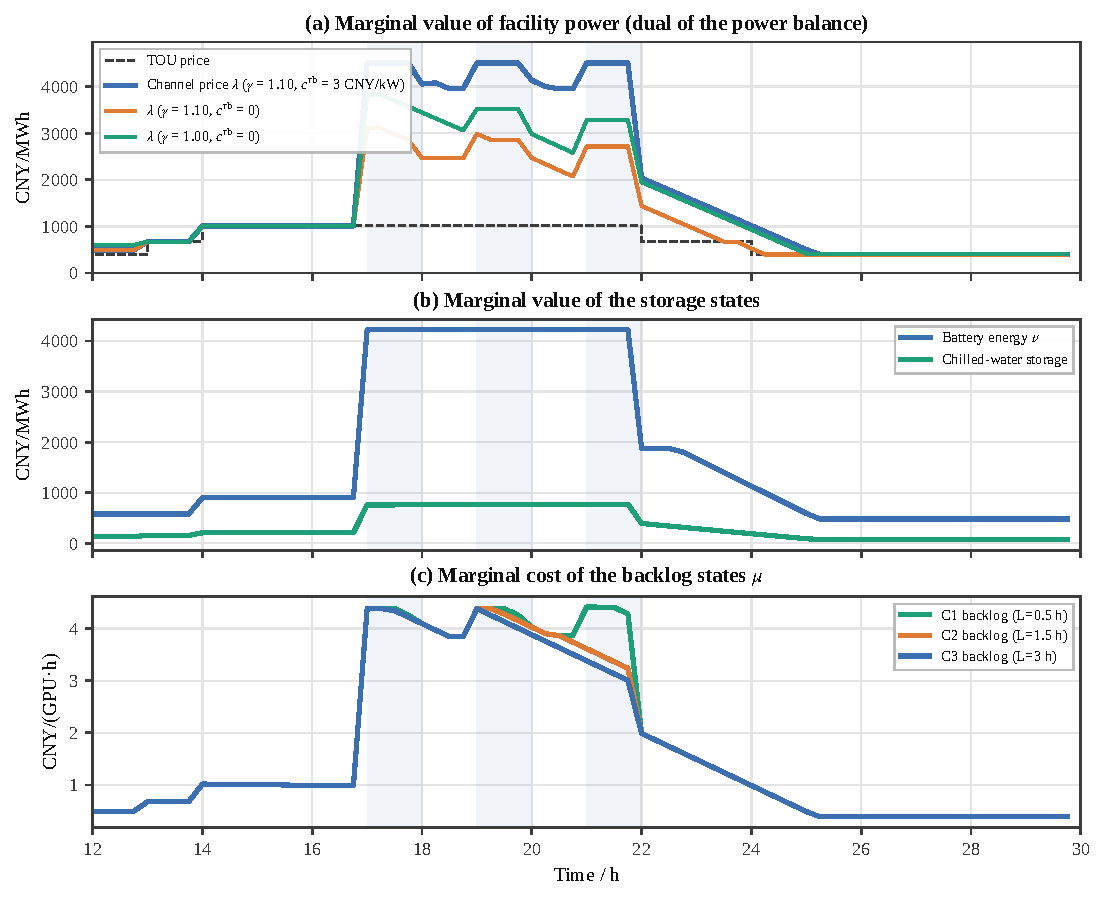
\includegraphics[width=0.80\textwidth]{fig08_shadow_prices.pdf}
\caption{Shadow prices of the joint plan (uniform 6~MW, perfect information). (a) Marginal value of facility electricity
(channel price); (b) marginal value of the storage states; (c) marginal cost of the backlog of each class.}
\label{fig:shadow}
\end{figure*}

\subsubsection{Cross-event capability region}
\label{sec:res-region}

The previous subsections compared strategies for given commitments. When bidding day-ahead, the data center needs to
know which commitment vectors $(C_1,C_2,C_3)$ it can deliver in full. Experiment~25 computes the capability region of
Proposition~\ref{prop:region} under perfect information along 91 rays $C=t\,d$ ($d$ on a simplex grid), together with the
deliverable sets of the benchmarks, the multi-event energy bound and the vertex certificate, for the base case (gap
1~h, $\gamma=1.10$) and a tight case (gap 0.5~h, $\gamma=1.00$). IR-O* uses the hindsight-optimal split for every ray,
the upper limit of any static split (\tabref{tab:region}, \figref{fig:region}).

\begin{table}[!t]
\caption{Capability region of the three events (perfect information).}
\label{tab:region}
\centering\footnotesize
\setlength{\tabcolsep}{1.5pt}
\begin{tabular}{@{}lcc@{}}
\toprule
 & \makecell{Base\\($\tau=1$~h, $\gamma=1.10$)} & \makecell{Tight\\($\tau=0.5$~h, $\gamma=1.00$)}\\
\midrule
Stand-alone capability $\Gamma^0_{1,2,3}$ (MW) & 8.18 / 7.98 / 7.90 & 8.18 / 8.05 / 8.06\\
Support $h_{123}$ of JR (sum of $\Gamma^0_k$) & 24.06 (24.06) & 19.43 (24.29)\\
Energy bound $\bar b$ (MWh) & \makecell{25.66 = 11.36 + 11.41\\ + 9.07 $-$ 6.17} & \makecell{19.57 = 11.58 + 11.40\\ + 2.93 $-$ 6.34}\\
Template $\mathcal T$ & exact (8 vertices) & $\theta^*=0.9997$ (10 vertices)\\
\makecell[l]{Uniform capability (MW):\\JR / IR-P+ / IR-O* / IR-O / IR-P} & \makecell{7.90 / 7.90 / 6.44 /\\ 5.50 / 4.52} & \makecell{6.48 / 6.47 / 6.44 /\\ 3.05 / 2.55}\\
\makecell[l]{Region volume relative to JR:\\IR-P+ / IR-O* / IR-O / IR-P} & \makecell{1.000 / 0.966 /\\ 0.770 / 0.279} & \makecell{0.850 / 0.962 /\\ 0.278 / 0.119}\\
\bottomrule
\multicolumn{3}{@{}p{0.97\columnwidth}@{}}{\scriptsize Energy bound = virtual storage + storage + channel + baseline difference.}
\end{tabular}
\end{table}

\begin{figure*}[!t]
\centering
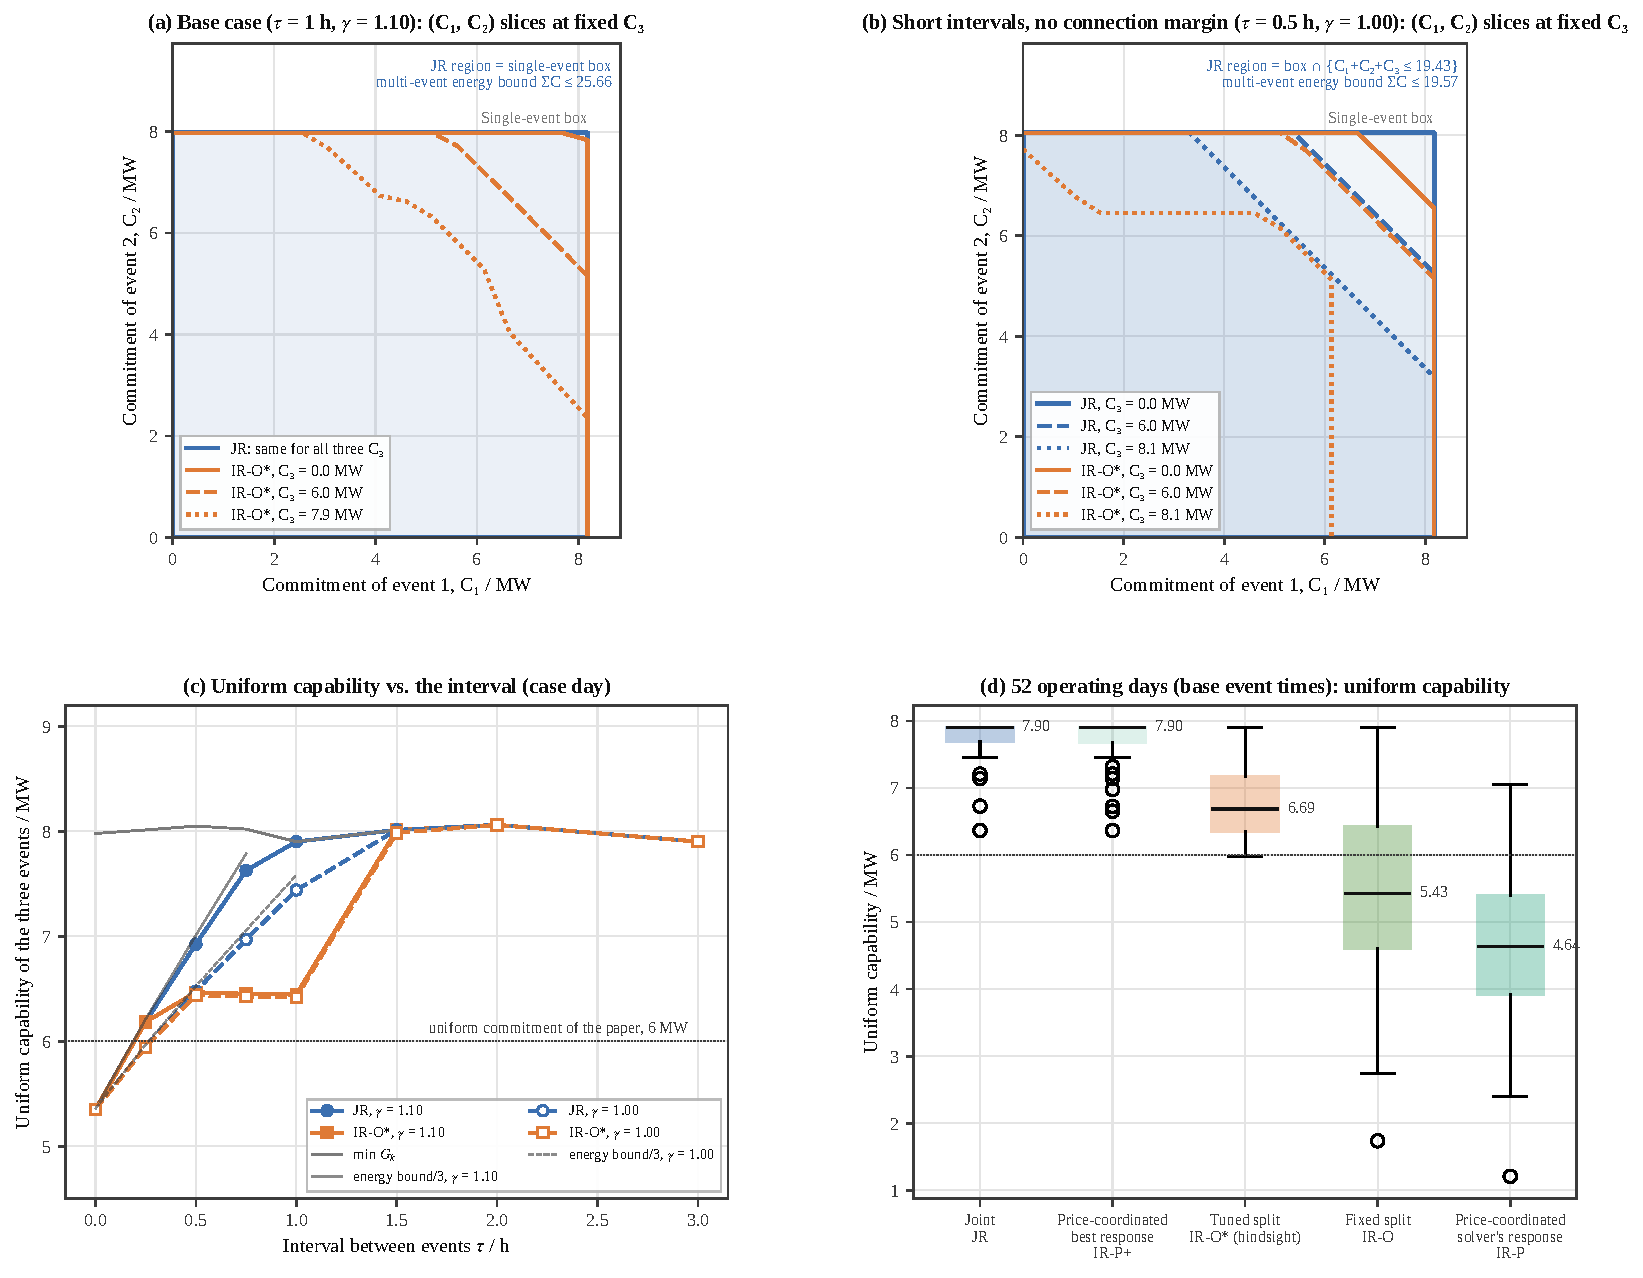
\includegraphics[width=0.86\textwidth]{fig28_region.pdf}
\caption{Cross-event capability region (perfect information). (a)(b) Slices $(C_1,C_2)$ at fixed $C_3$: joint recovery
(shaded, exact by the vertex certificate), IR-O* with the hindsight-optimal split for every commitment vector (lines),
and the single-event box (grey); (c) uniform capability of the three events versus the gap ($\gamma=1.10$ solid, $1.00$
dashed) with the minimum stand-alone capability and one third of the energy bound; (d) uniform capability on the 52
operating days, where IR-P+ is the most favourable and IR-P the solver's response to the price.}
\label{fig:region}
\end{figure*}

The capability region of joint recovery is the single-event box intersected with one total-energy cut. In both cases,
the support of every pair of events equals the sum of their stand-alone capabilities, so two events never conflict;
only the total of the three events can fall below the sum, which gives the single coupling cut $C_1+C_2+C_3\le h_{123}$
(each event lasts 1~h). In the base case, $h_{123}$ equals the sum of the stand-alone capabilities and the region is the
box itself, so the three events are independent; in the tight case the cut removes a corner of the box. This is the
virtual battery of Proposition~\ref{prop:region}: event power limits $\Gamma^0_k$ and one cross-event energy budget
$h_{123}$. All eight vertices of the template are deliverable in the base case, so the description is exact; in the
tight case one vertex falls marginally short ($\theta^*=0.9997$), \ie\ the template differs from the true region by
less than 0.03\%.

The multi-event energy bound is tight: it holds in all 24 gap--margin cases and on all 52 days, and where the cut is
active (14 cases and 18 days) it exceeds the exact LP value by 0.02--0.71~MWh ($\le$3.0\%). On the case day the evening load
without response and storage actions exceeds the baseline by about 2.2~MW, so the baseline difference $\Delta$ of the three events
is $-6.2$ to $-6.7$~MWh for gaps up to 1~h, a non-negligible part of the budget that the unbiased-baseline assumption
of Proposition~\ref{prop:bound} would ignore (the bound would overestimate by 42\% at a zero gap).

Independent recovery shrinks the cross-event energy budget rather than the stand-alone capabilities. In the base case
IR-O* reaches the JR boundary in every single-event and two-event direction, and the loss concentrates in the corner
where all three commitments are high: the maximum total commitment along the same rays is 19.33 against 23.70~MW
($-18.4\%$) and the uniform capability 6.44 against 7.90~MW ($-18.4\%$), although the volume is only 3.4\% smaller. The
fixed split IR-O loses more (volume $-23\%$, uniform capability 5.50~MW). In the tight case the channel is narrow
anyway and IR-O* nearly coincides with JR (Corollary~\ref{cor:novalue}(c)), but in directions with only two committed
events it still loses up to 11\%.

A price signal alone is not enough. The optimal IT response to the channel price is not unique, and the response
picked by the solver (IR-P) delivers only 53--82\% of JR along the rays of the base case (28\% of the volume) and 60\%
of the uniform capability of JR on average over the 52 days. Selecting the most favourable exactly optimal response
(IR-P+) reaches the JR boundary on all rays of the base case but only on 59\% of the rays of the tight case; with
$\gamma=1.00$ and gaps of 1.5--3~h no exactly optimal response is deliverable (uniform capability 4.97--5.72~MW against
7.90--8.06~MW for JR). Allowing the IT side to be 0.1\% suboptimal recovers the JR capability in all 24 cases and on all
52 days, except for up to 5\% in some directions of the tight case; the residual gap arises because the IT model
estimates its power budget with idle storage and converts cooling with the electric-chiller COP, so the joint price is
only an approximate supporting price for it. The channel price thus contains almost all the information needed but
does not select a deliverable plan: the IT side must also know which of its many near-optimal plans to choose.

The uniform capability of JR increases almost linearly with the gap and follows the energy bound
(\figref{fig:region}(c)). At a zero gap, JR, IR-O* and IR-P+ coincide (5.35~MW), since nothing can be recovered between
the events. JR reaches the stand-alone capability at a gap of 1~h with $\gamma=1.10$ and 1.5~h with $\gamma=1.00$; at a
gap of 1~h its uniform capability is 7.44/7.88/7.90~MW for $\gamma$ = 1.00/1.05/1.10. IR-O* stays at about 6.4~MW for gaps
of 0.5--1~h, because it spends the channel on unnecessary catch-up, and catches up with JR only from 1.5~h, which is the
difference of the minimum recovery gaps of Theorem~\ref{thm:closed} on the capability region. Over the 52 days the
uniform capability of JR averages 7.75~MW (6.37--7.90); relative to JR, IR-P+ achieves 99.4\%, IR-O* 88.6\% (80--100\%),
IR-O 71\% and IR-P 60\%, and the energy cut is active on 18 days.

For bidding, the current practice of one value per event requires the uniform capability to guarantee delivery under
any call pattern: 7.90~MW per event in the base case and 6.48~MW in the tight case. If the data center instead declares
the virtual-battery parameters (three $\Gamma^0_k$ and the budget $h_{123}$, four numbers), the grid operator may call
any combination within them; in the tight case, two calls of up to 8.0~MW each become possible, 24\% more than the
uniform declaration, while three calls may total at most 19.43~MW. Under independent recovery the same declaration
needs a further discount: the energy budget of IR-O* is 18\% lower than that of JR in the base case.

\subsubsection{Distributed coordination by plan--price exchange}
\label{sec:res-admm}

The previous subsection showed that a one-shot channel price does not determine a deliverable plan. Experiment~26 lets
the IT scheduler and the facility controller keep their own models, states and forecasts and exchange only the
deferrable power plan (one number per step) and the price, iterating \eqref{eq:admm} on the same joint model
(Proposition~\ref{prop:admm}); the facility side requires every called event to be valid and $\rho=200$~CNY per
MW$^2$ and step unless stated otherwise (\figref{fig:admm}).

\begin{figure*}[!t]
\centering
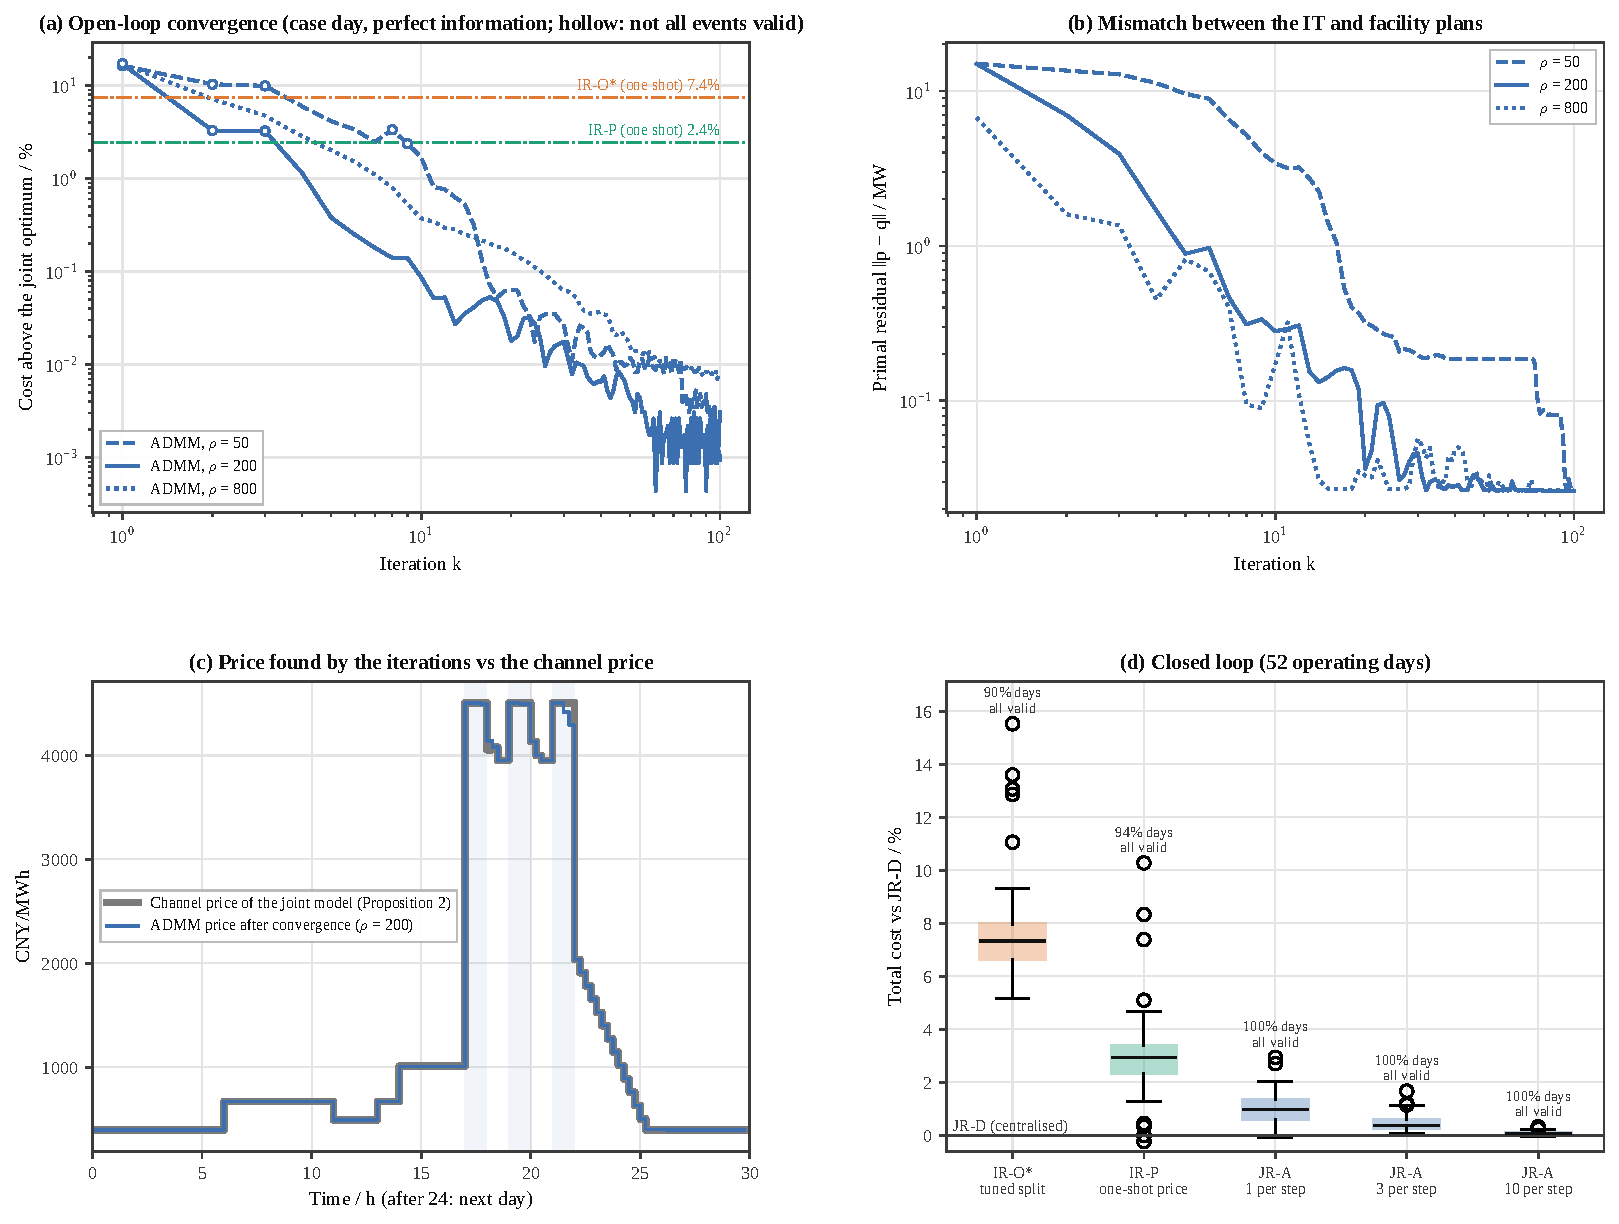
\includegraphics[width=0.86\textwidth]{fig29_admm.pdf}
\caption{Distributed joint recovery by plan--price exchange. (a) Open-loop cost of implementing the IT side's plan
relative to the joint optimum (log--log; hollow: not all events valid), with the one-shot benchmarks IR-P and IR-O*;
(b) mismatch between the two plans; (c) price after convergence ($\rho=200$) and channel price of the joint model
(shaded: events); (d) closed-loop cost relative to the centralised JR-D on 52 operating days and share of days with all
events valid.}
\label{fig:admm}
\end{figure*}

In open loop (case day, perfect information, uniform 6~MW), the relevant measure is the cost of implementing the IT
side's current plan, \ie\ the total cost when the facility responds optimally to it. With $\rho=200$ this cost falls
below that of the one-shot price coordination IR-P (2.44\% above the joint optimum) from the fourth iteration on, and
lies 0.38\%, 0.09\% and 0.02\% above the optimum after 5, 10 and 20 iterations; IR-O* with the hindsight-optimal split
is 7.38\% above. The iteration starts from the nominal IT load, and the IT plans of the first three iterations do not yet
keep all events valid: a few exchanges are needed to move catch-up out of the scarce hours. A small $\rho$ updates the
price slowly ($\rho=50$: better than IR-P from iteration 10, within 0.1\% from iteration 17), and a large one locks
the plans early ($\rho=800$: iterations 5 and 26). After 100 iterations the residual stays at about 0.03~MW, the
resolution of the tangent cuts, and the implemented cost is within 0.001--0.008\% of the optimum.

The price found by the iteration is the channel price (\figref{fig:admm}(c)). After convergence it differs from the
channel price of the joint model (Proposition~\ref{prop:price}) by less than 1~CNY/MWh in 79\% of the steps, and it
reproduces the price of about 4,500~CNY/MWh during the events and its gradual decline afterwards; only three steps at
the beginning and end of the events differ more (up to 214~CNY/MWh). The iteration discovers the channel price without
any party solving the joint model and broadcasting it.

In closed loop, the centralised JR-D costs $22.84\times10^4$~CNY on the case day, and JR-A with 1, 3 and 10 iterations
per MPC step costs $+0.67\%$, $+0.22\%$ and $+0.03\%$ more; with three iterations, $\rho$ = 50, 200 and 800 differ by
less than 0.1\%. Over the 52 days, JR-A costs $+0.99\%$, $+0.45\%$ and $+0.09\%$ more than JR-D with 1, 3 and 10
iterations and keeps all events valid on every day, whereas IR-P costs $+2.97\%$ more (all events valid on 94\% of the
days). One exchange per step thus recovers 67\% of the advantage of joint recovery over the strongest independent
benchmark, three exchanges 85\% and ten 97\%. A full day takes about 6~s for JR-D and 12/29/88~s for JR-A with
1/3/10 iterations, less than 1~s per step. Joint recovery therefore does not require merging the IT scheduler and the
facility energy management system: both keep their own models and data, provided that plans and prices are exchanged in
both directions a few times per 15~min.

\subsection{Day-ahead commitment under uncertainty}
\label{sec:res-dayahead}

\subsubsection{Commitment--operation pairing}
\label{sec:res-pairing}

Three commitments are compared on the case day and 20 operating days, each operated by IR-O* (with $\alpha$ re-tuned
for that commitment) and by JR-D: the single-event capability assessment (SE), the SE commitment scaled by the
back-tested factor $\theta^*=0.8$ (SE-$\theta$, a cautious conventional practice), and the coupled day-ahead commitment
(DA) (\tabref{tab:pairing}, \figref{fig:pairing}).

\begin{table}[!t]
\caption{Commitment--operation pairing (20 operating days): fulfilment / days with all events valid / mean cost
($10^4$~CNY).}
\label{tab:pairing}
\centering\footnotesize
\setlength{\tabcolsep}{2.8pt}
\begin{tabular}{@{}llcc@{}}
\toprule
Commitment (sum, MW) & Setting & IR-O* & \textbf{JR-D}\\
\midrule
SE 8.18/7.98/7.90 (24.1) & $\crb=3$ & 81.8\% / 45\% / 25.63 & 96.0\% / 95\% / 23.06\\
SE-$\theta$ 6.54/6.38/6.32 (19.2) & $\crb=3$ & 97.5\% / 95\% / 24.08 & 99.9\% / 100\% / 22.44\\
DA 3.27/6.65/7.90 (17.8) & $\crb=3$ & 97.0\% / 100\% / 23.79 & \textbf{98.8\% / 100\% / 22.39}\\
SE = DA 8.18/7.98/7.90 & $\crb=0$ & 84.3\% / 45\% / 21.43 & 96.0\% / 95\% / 19.18\\
SE-$\theta$ 6.54/6.38/6.32 & $\crb=0$ & 98.2\% / 95\% / 19.60 & \textbf{99.7\% / 100\% / 18.85}\\
\bottomrule
\end{tabular}
\end{table}

\begin{figure*}[!t]
\centering
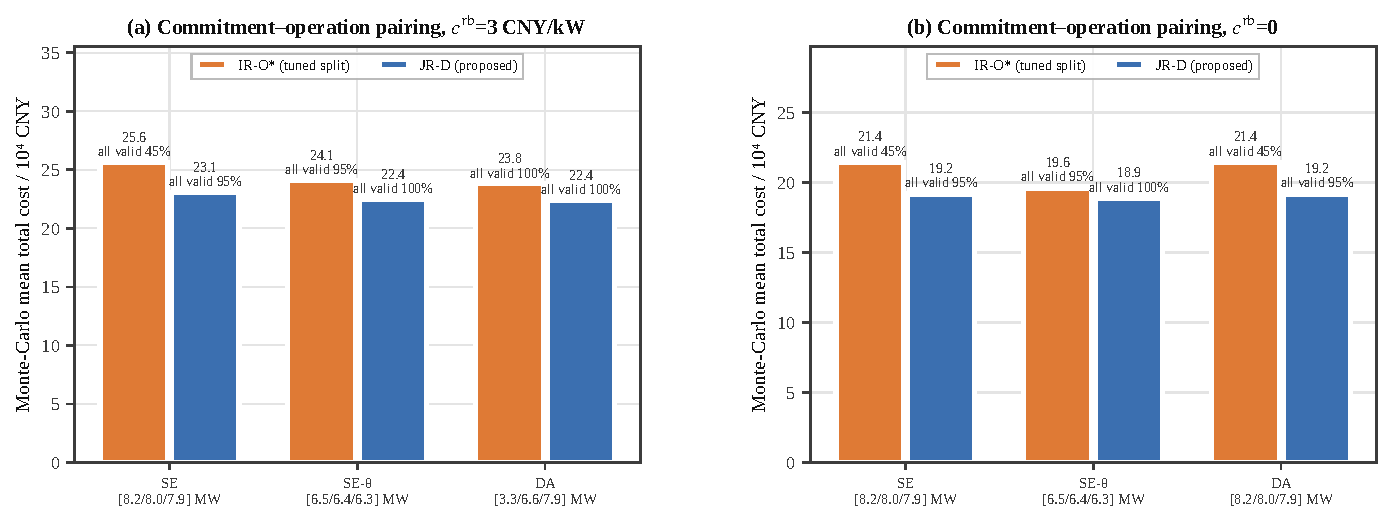
\includegraphics[width=0.86\textwidth]{fig09_commitment.pdf}
\caption{Commitment--operation pairing: mean total cost over 20 operating days with the share of days on which all
three events are valid.}
\label{fig:pairing}
\end{figure*}

The current practice, a single-event assessment operated by independent recovery (SE with IR-O*), keeps all three events
valid on only 45\% of the days. The coupled commitment operated by joint recovery (DA with JR-D) keeps them valid on
every day at a 12.6\% lower cost. Changing only the commitment to DA reduces the cost by 7.2\% (DA with IR-O*), and
operating the DA commitment by JR-D reduces it by a further 5.9\%. In the rebound-priced setting the coupled model
commits less in E1 and keeps the channel for the better-paid E3. In the rule setting the coupled commitment coincides
with the single-event capabilities, and the scaled SE-$\theta$ commitment is better for both operating strategies
because the five day-ahead scenarios cover the high-load tail of the operating days poorly; the risk-averse commitment
below addresses this.

\subsubsection{Risk-averse commitments}
\label{sec:res-risk}

Using ten historical joint scenarios and $\crb=3$, each risk setting of Proposition~\ref{prop:dro} yields a set of
commitments, which JR-D then operates out of sample on the same 52 days (\tabref{tab:risk}, \figref{fig:risk}).

\begin{table}[!t]
\caption{Risk-averse day-ahead commitments evaluated out of sample by JR-D on 52 days.}
\label{tab:risk}
\centering\footnotesize
\setlength{\tabcolsep}{2.8pt}
\begin{tabular}{@{}lcccc@{}}
\toprule
Setting & \makecell{E1/E2/E3 (sum)\\(MW)} & \makecell{Mean\\($10^4$~CNY)} & \makecell{Worst 10\%\\($10^4$~CNY)} & All valid\\
\midrule
SP ($\delta=0$) & 3.66/6.34/7.90 (17.9) & 22.50 & 27.33 & 100\%\\
DRO $\delta=0.2$ & 2.66/6.01/7.90 (16.6) & 22.47 & 27.27 & 100\%\\
DRO $\delta=0.4$ & 2.80/5.06/7.90 (15.8) & 22.45 & 27.24 & 100\%\\
\textbf{DRO $\delta=1.2$} & 0.96/5.77/7.90 (14.6) & \textbf{22.44} & \textbf{27.22} & 100\%\\
RO ($\delta=2$) & 4.54/2.17/7.90 (14.6) & 22.45 & 27.22 & 100\%\\
CVaR$_{0.8}$ & 4.22/2.50/7.90 (14.6) & 22.45 & 27.22 & 100\%\\
Mean--CVaR$_{0.9}$ ($w=0.5$) & 2.74/5.50/7.90 (16.1) & 22.46 & 27.26 & 100\%\\
Single-event assessment & 8.18/7.98/7.90 (24.1) & 23.11 & 29.12 & 96.2\%\\
\bottomrule
\end{tabular}
\end{table}

\begin{figure*}[!t]
\centering
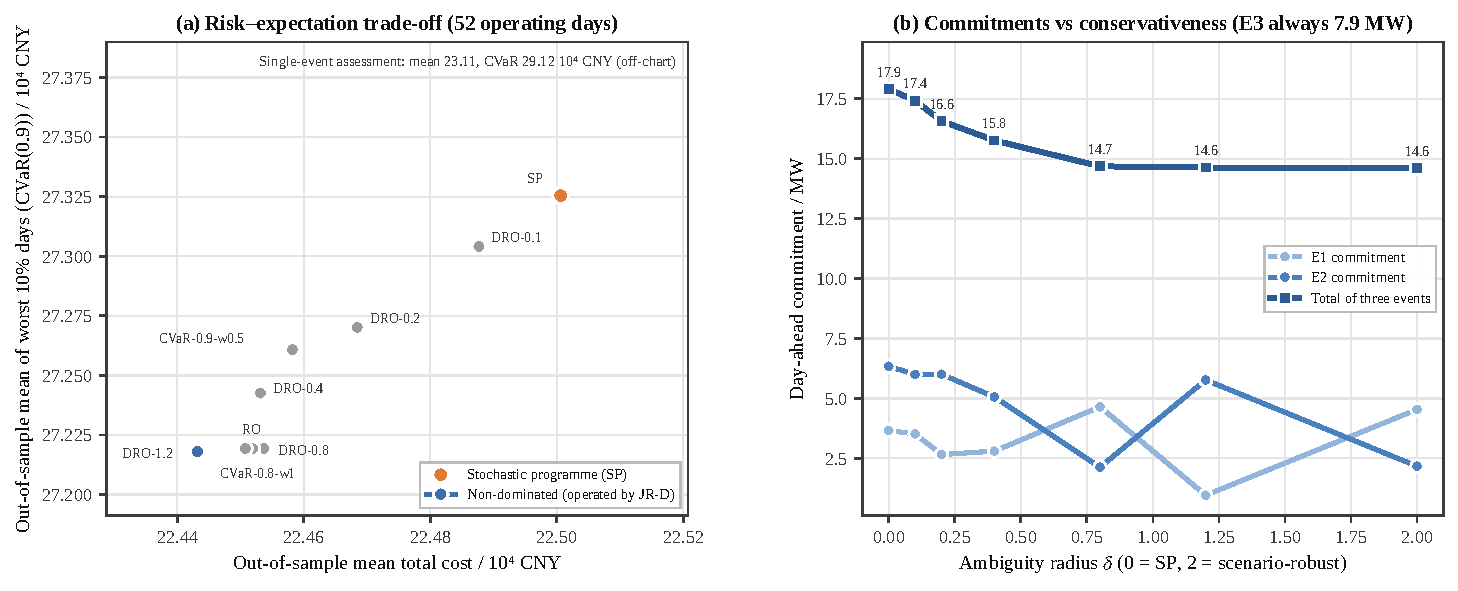
\includegraphics[width=0.86\textwidth]{fig15_risk_pareto.pdf}
\caption{Risk-averse commitments. (a) Out-of-sample mean and mean of the worst 10\% of days for each risk setting on the
52 days (the single-event assessment lies outside the chart); (b) commitments versus the ambiguity radius $\delta$.}
\label{fig:risk}
\end{figure*}

A higher conservativeness lowers the total commitment: as $\delta$ increases from 0 to 0.8, the sum falls monotonically
from 17.9 to 14.7~MW and then stays constant. The best-paid E3 is always committed at its capability of 7.9~MW and the
reduction falls on E1 and E2, between which the model is nearly indifferent, so their split is not unique
(\figref{fig:risk}(b)). The distributionally robust commitments lower both the mean and the tail out of sample: compared
with SP, $\delta$ = 0.4--1.2 reduces the mean by 0.21--0.26\% and the mean of the worst 10\% of days by 0.3--0.4\%, all
paired differences being significant (Wilcoxon $p\le2\times10^{-4}$). $\delta=1.2$ is best in both measures and is the
non-dominated knee point of \figref{fig:risk}(a). The reason is that the ten historical scenarios cover the high-load tail
of the operating days poorly, so SP commits too much and earns less and pays more on adverse days, which the robust
commitments avoid by committing less in E1 and E2. The improvement is small, which shows that coupled commitment with
joint recovery is already robust. Coupled commitments are far better than the single-event assessment, which costs 2.7\%
more on average and 6.6\% more on the worst 10\% of days, with all events valid on only 96.2\% of the days. The DRO
model adds only 21 continuous variables and 30 constraints and solves in 14--25~s with ten scenarios, against 10~s for SP.

\subsubsection{Scenario generation and seasonal drift}
\label{sec:res-scen}

The base commitment uses five equally likely quantile scenarios. Experiment~23 replaces them by K-means scenarios with
non-uniform probabilities ($K$ = 5, 10, 20) and builds a DRO ball with $\delta=0.4$ around them; JR-D then operates each
commitment on the 52 out-of-sample days (\tabref{tab:scen}, \figref{fig:ext}(b)--(d)).

\begin{table}[!t]
\caption{Scenario generation: commitments and costs (52 days, operated by JR-D; costs in $10^4$~CNY).}
\label{tab:scen}
\centering\footnotesize
\setlength{\tabcolsep}{2.4pt}
\begin{tabular}{@{}lccccc@{}}
\toprule
Scenarios & \makecell{E1/E2/E3\\(MW)} & \makecell{In-\\sample} & \makecell{Out-of-\\sample} & \makecell{vs\\quantile-5} & \makecell{In-sample\\underestimate}\\
\midrule
Quantile-5 & 3.27/6.65/7.90 & 19.92 & 22.50 & -- & 13.0\%\\
K-means-5 & 2.42/5.63/7.90 & 20.96 & 22.45 & $-0.19\%$ & 7.1\%\\
K-means-10 & 3.69/4.72/7.90 & 20.68 & 22.46 & $-0.15\%$ & 8.6\%\\
K-means-20 & 3.73/5.51/7.90 & 20.22 & 22.48 & $-0.07\%$ & 11.2\%\\
K-means-5 + DRO & 0.92/6.32/7.90 & 21.10 & 22.45 & $-0.23\%$ & 6.4\%\\
K-means-10 + DRO & 4.71/2.99/7.90 & 20.86 & 22.46 & $-0.19\%$ & 7.6\%\\
\bottomrule
\end{tabular}
\end{table}

\begin{figure*}[!t]
\centering
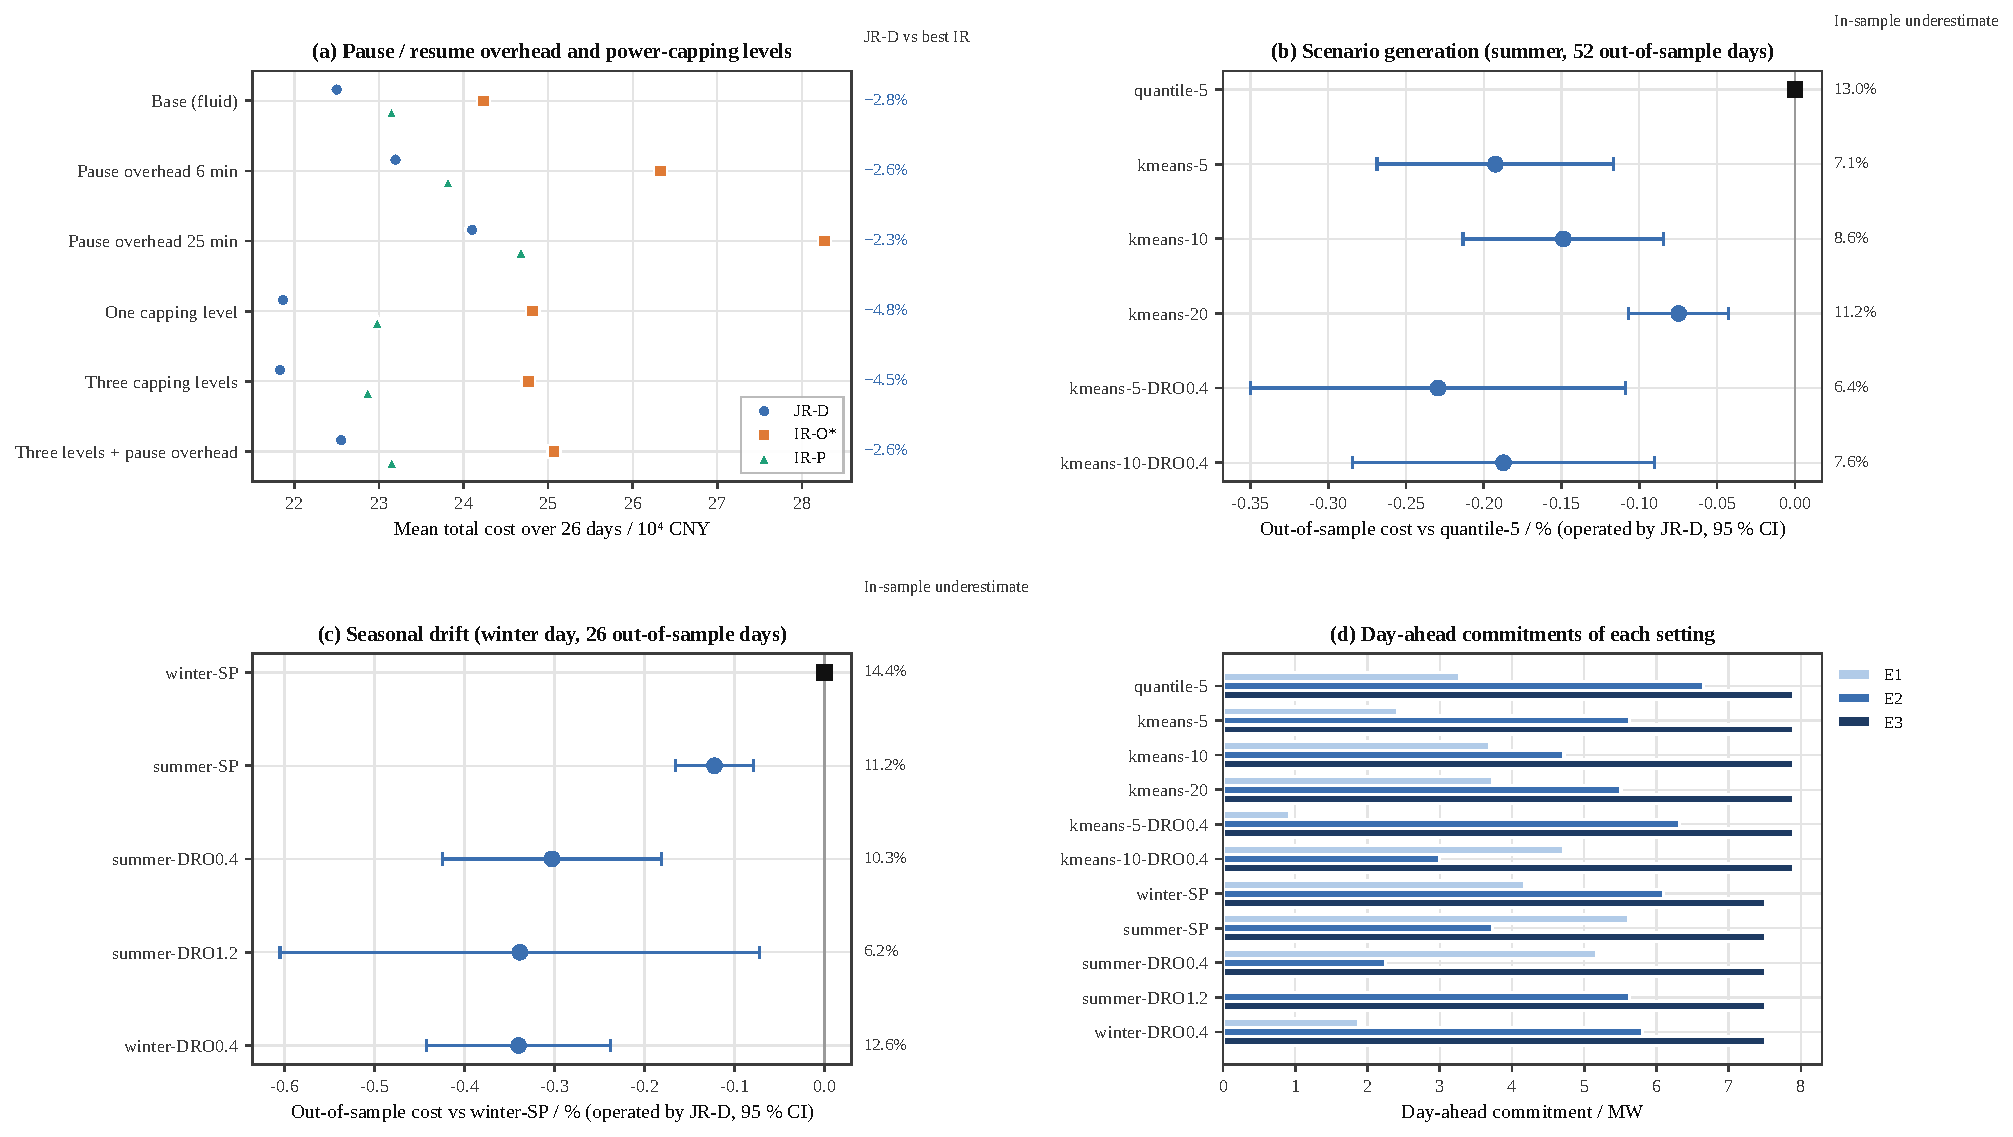
\includegraphics[width=0.96\textwidth]{fig25_extensions.pdf}
\caption{(a) Pause/resume overheads and power-capping levels: mean total cost on 26 operating days (right: JR-D relative
to the strongest independent benchmark); (b)(c) scenario generation and seasonal drift: paired out-of-sample cost
difference to the reference setting (95\% CI; right: underestimate of the in-sample estimate); (d) day-ahead
commitments of each setting.}
\label{fig:ext}
\end{figure*}

The out-of-sample cost is nearly insensitive to scenario generation: the six settings differ by less than 0.23\% and
keep all events valid on every day, although the commitments differ widely (E1 from 0.9 to 4.7~MW, E2 from 3.0 to
6.7~MW). The cost is therefore flat around the optimal commitment, consistent with \secref{sec:res-risk}; the K-means
improvements are statistically significant (Wilcoxon $p\le3\times10^{-5}$) but negligible in size. In-sample estimates
are optimistic by 6--13\%, mainly because the day-ahead model optimises each scenario with perfect information whereas the
operation has only forecasts; K-means-5/10 and DRO reduce the bias to 6--9\%, but 20 scenarios raise it again to 11\%.
Revenue estimates for bidding and investment appraisals should therefore rely on the out-of-sample cost of rolling
operation. A seasonal drift matters little: when the winter case day (10 January 2025) builds its scenarios from the
summer weather pool instead of the winter pool, the commitments change markedly (\figref{fig:ext}(d)) but the cost on 26
out-of-sample winter days is 0.12\% lower rather than higher, with all events valid every day, and DRO with
$\delta$ = 0.4/1.2 lowers it consistently by about 0.3\%.

\subsection{Sensitivity analysis}
\label{sec:res-sens}

To evaluate the robustness of the conclusions under different operating conditions and policy settings, this subsection
varies the commitment and system margins, the settlement and policy parameters, the realism of the model and the
external conditions.

\subsubsection{Commitment level, event gap and connection margin}
\label{sec:sens-commit}

Under perfect information, with IR-O* using the hindsight-optimal split and IR-P the perfect-information shadow price,
\figref{fig:sens} varies the event duration, gap, connection margin and commitment, and \figref{fig:map} maps the cost
reduction on the gap--margin plane; \tabref{tab:sens} lists the commitment sweep.

\begin{table}[!t]
\caption{Commitment sweep under perfect information: fulfilment / total cost ($10^4$~CNY).}
\label{tab:sens}
\centering\footnotesize
\setlength{\tabcolsep}{3pt}
\begin{tabular}{@{}llcccc@{}}
\toprule
Commitment & Setting & IR-O* (hindsight) & IR-P & \textbf{JR} & JR vs best\\
\midrule
6~MW & $\crb=0$ & 100\% / 19.91 & 100\% / 19.92 & 100\% / 19.31 & $-3.0\%$\\
7~MW & $\crb=0$ & 92.1\% / 20.43 & 88.8\% / 20.60 & \textbf{100\% / 19.04} & $-6.8\%$\\
8~MW & $\crb=0$ & 79.8\% / 22.27 & 77.7\% / 22.23 & \textbf{99.5\% / 19.09} & $-14.1\%$\\
9~MW & $\crb=0$ & 71.6\% / 23.23 & 69.0\% / 23.25 & 89.1\% / 20.06 & $-13.7\%$\\
8~MW & $\crb=3$ & 74.5\% / 26.76 & 92.9\% / 24.07 & \textbf{99.5\% / 23.09} & $-4.1\%$\\
\bottomrule
\end{tabular}
\end{table}

\begin{figure*}[!t]
\centering
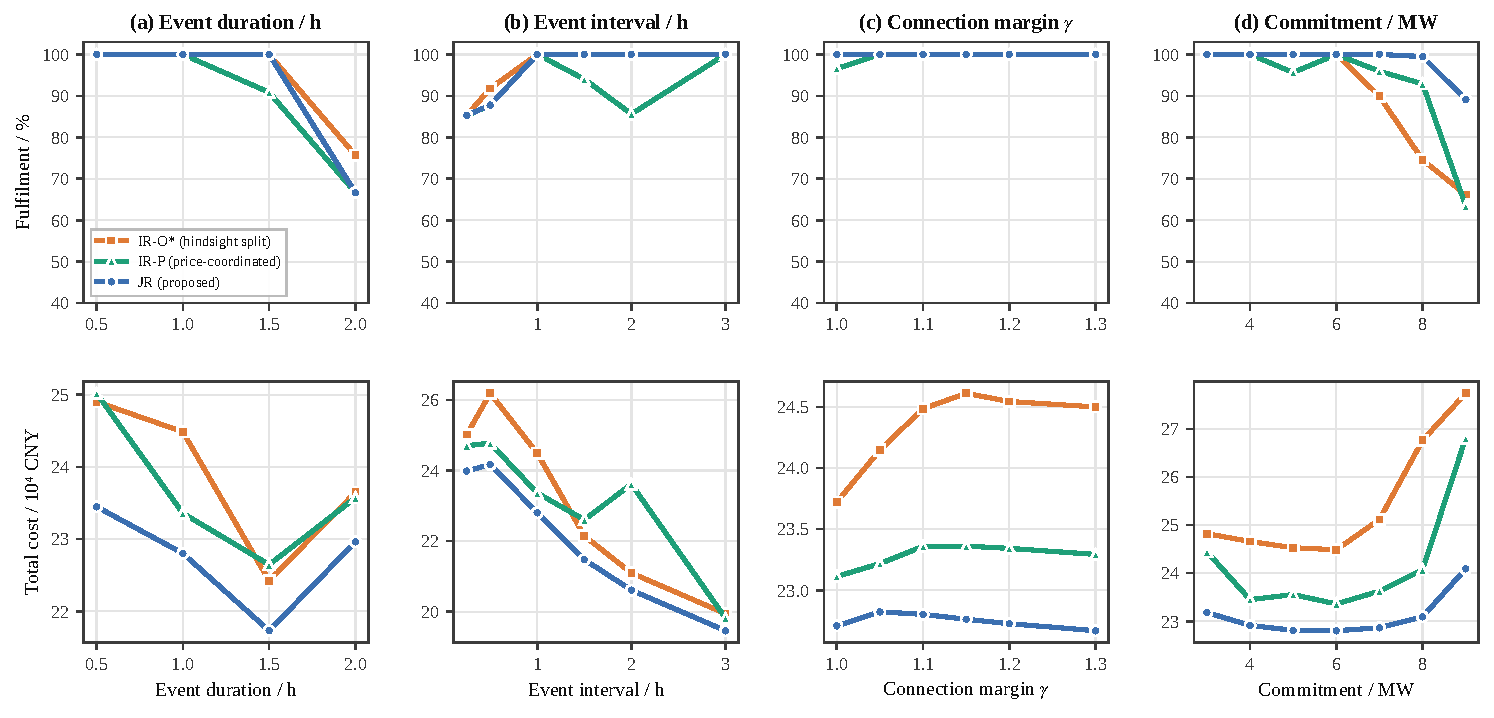
\includegraphics[width=0.96\textwidth]{fig05_sensitivity.pdf}
\caption{Sensitivity under perfect information ($\crb=3$~CNY/kW): fulfilment (top) and total cost (bottom) versus (a)
event duration, (b) event gap, (c) connection margin and (d) uniform commitment. The rule setting is shown in
\figref{fig:sens0}.}
\label{fig:sens}
\end{figure*}

\begin{figure*}[!t]
\centering
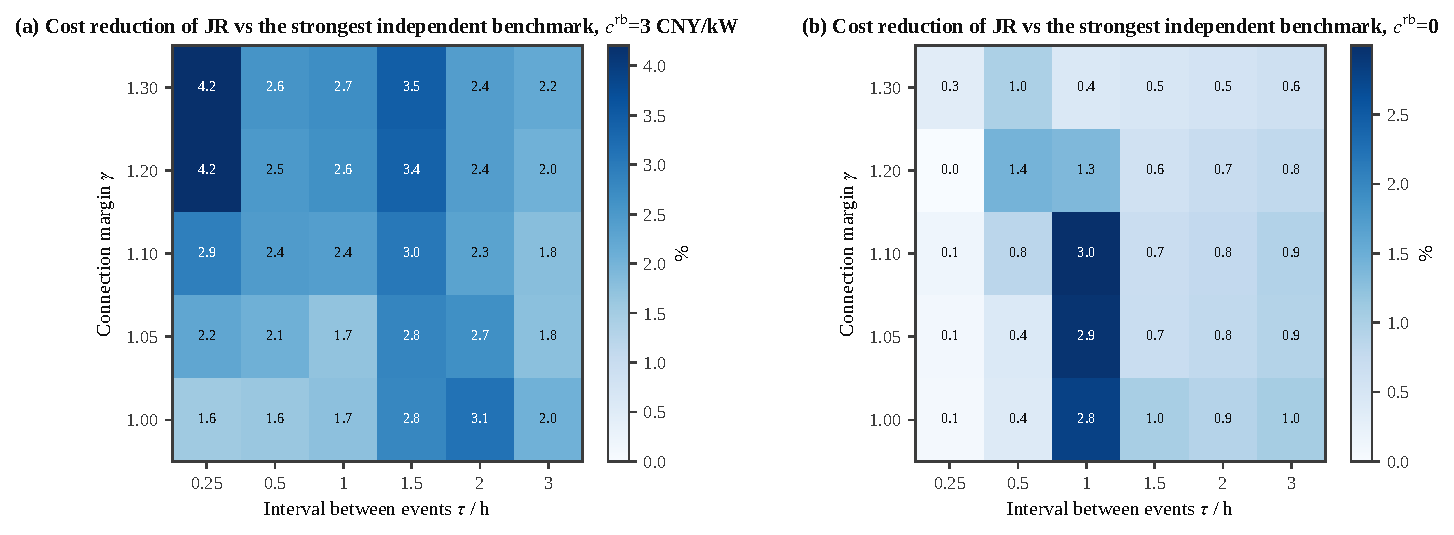
\includegraphics[width=0.94\textwidth]{fig06_interval_capacity_map.pdf}
\caption{Cost reduction of JR relative to the stronger of IR-O* and IR-P on the gap--margin plane: (a) rebound-priced
setting, (b) rule setting.}
\label{fig:map}
\end{figure*}

Deliverable capacity is the main value of joint recovery. With the requirement of $\ge$99\% fulfilment, even
hindsight-tuned independent recovery can commit only about 6~MW per event, whereas JR can commit about 8~MW (+33\%); at
8~MW, JR fulfils 99.5\% against less than 80\% for the best benchmark in the rule setting, at a 14.1\% lower cost. With
moderate commitments (6~MW) the advantage is only 2--3\%. On the gap--margin plane the reduction in the rule setting is
0--3.0\%, with the peak at a gap of 1~h and $\gamma\le1.10$ (2.8--3.0\%) and generally at most 1.4\% for gaps of 0.5~h
or less or 1.5~h or more; in the rebound-priced setting it is 1.6--4.2\% and never negative. Corollary~\ref{cor:novalue}
explains why the advantage first rises and then falls with the channel width: with a too narrow channel neither strategy
recovers, with a wide one both do.

Fulfilment is not what joint recovery maximises. With a gap of 0.5~h and $\crb=3$, JR fulfils 4--6 points less than
IR-O* but at a lower cost: the optimum delivers slightly above the 80\% validity threshold in some events to reduce the
rebound charge. With 2-h events, all three methods keep only two events valid. Both effects are cross-event trade-offs
induced by the Jiangsu settlement (80\% threshold, 120\% cap). Correcting the IT budget of the benchmarks
(\secref{sec:strategies}) has little effect under perfect information: at 6~MW the costs of IR-O* and IR-P drop by only
$0.06$--$0.07\times10^4$~CNY and the capacity conclusions are unchanged; the correction matters mainly for closed-loop
operation on heavy-load days.

\subsubsection{Rebound charge and DR payment}
\label{sec:sens-rebound}

\tabref{tab:rebound} and \figref{fig:rebound} treat the rebound charge as a policy parameter (case day, uniform 6~MW,
deterministic rolling operation). As the charge rises, the maximum rebound of JR-D after the events falls smoothly from
6.52 to 2.98~MW, its fulfilment stays at 100\% up to 4~CNY/kW, and JR-D is the cheapest strategy at every charge. IR-P
cuts the rebound to 2.04~MW at 6~CNY/kW, but its fulfilment drops to 65.9\%. On the plane of cost (excluding the rebound
charge) against maximum rebound, the trade-off curve of JR-D lies to the lower left of the benchmarks
(\figref{fig:rebound}(a)): controlling the rebound while keeping the events valid requires a joint allocation of the
channel. Without a rebound charge, however, joint recovery does not suppress the rebound by itself, since all strategies
raise the import to near the connection limit; whether and at which price to charge rebound is a policy choice of the
grid operator or aggregator, and joint recovery minimises its cost.

\begin{table}[!t]
\caption{Rebound charge as a policy parameter (case day, uniform 6~MW).}
\label{tab:rebound}
\centering\footnotesize
\setlength{\tabcolsep}{3pt}
\begin{tabular}{@{}lccccccc@{}}
\toprule
$\crb$ (CNY/kW) & 0 & 0.5 & 1 & 2 & 3 & 4 & 6\\
\midrule
JR-D max rebound (MW) & 6.52 & 6.47 & 6.45 & 6.31 & 5.77 & 5.27 & 2.98\\
JR-D cost ($10^4$~CNY) & 19.34 & 20.12 & 20.83 & 22.02 & 22.84 & 23.47 & 24.47\\
Best benchmark ($10^4$~CNY) & 19.97 & 20.79 & 21.57 & 22.60 & 23.61 & 24.48 & 25.88\\
& \scriptsize IR-O* & \scriptsize IR-O* & \scriptsize IR-O* & \scriptsize IR-P & \scriptsize IR-P & \scriptsize IR-P & \scriptsize IR-P\\
JR-D vs best & $-3.2\%$ & $-3.3\%$ & $-3.4\%$ & $-2.6\%$ & $-3.3\%$ & $-4.1\%$ & $-5.5\%$\\
\bottomrule
\end{tabular}
\end{table}

\begin{figure*}[!t]
\centering
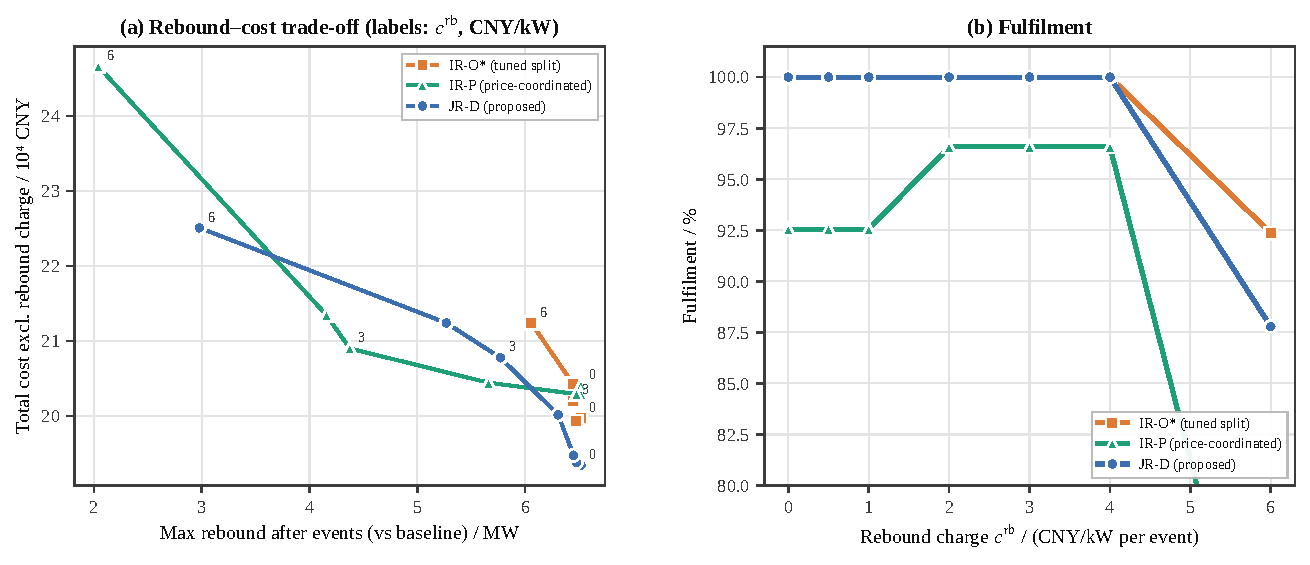
\includegraphics[width=0.84\textwidth]{fig10_rebound_pareto.pdf}
\caption{Rebound charge as a policy parameter. (a) Trade-off between the cost excluding the rebound charge and the
maximum rebound (labels: $\crb$ in CNY/kW); (b) fulfilment versus the rebound charge.}
\label{fig:rebound}
\end{figure*}

Across the nine combinations of DR payment (1--3~CNY/kWh) and shortfall coefficient ($\kappa$ = 0.5--2), JR-D is
always the cheapest, by 1.5\% (1~CNY/kWh, $\kappa=0.5$) to 4.0\% (3~CNY/kWh, $\kappa=2$) against the strongest benchmark
(\figref{fig:robust}(a)): the higher the payment and the stricter the shortfall assessment, the more valuable joint
recovery. At 1~CNY/kWh all three optimised strategies respond only partially (JR-D fulfils 33--88\%), since keeping
most events valid is no longer worthwhile.

\begin{figure*}[!t]
\centering
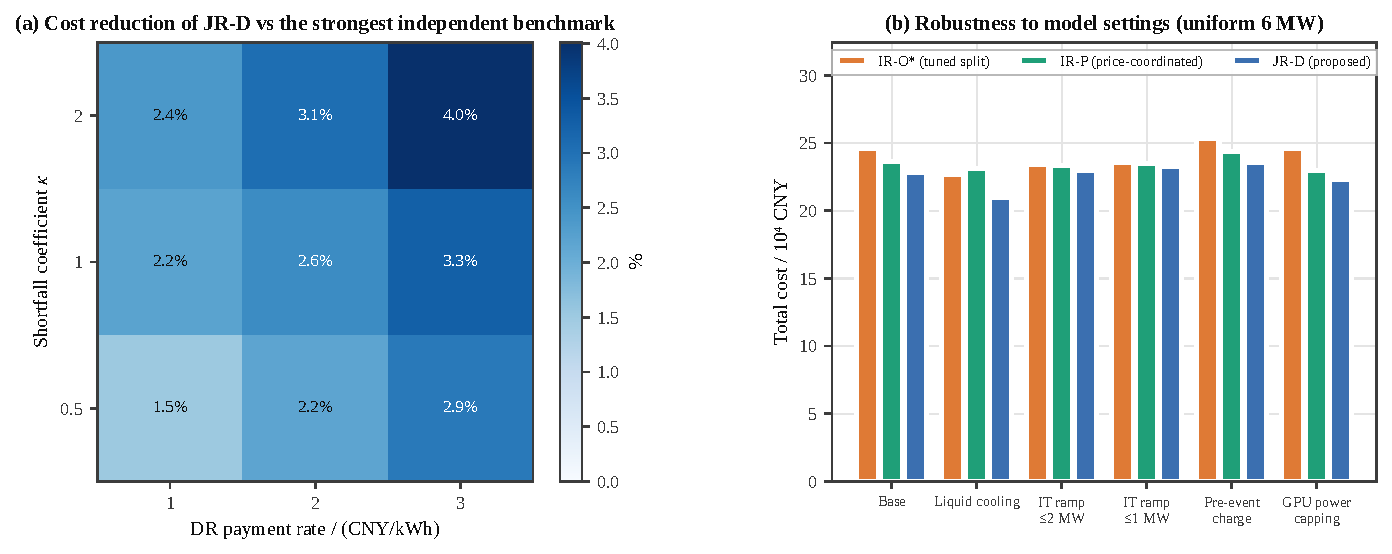
\includegraphics[width=0.90\textwidth]{fig13_robustness.pdf}
\caption{(a) Cost reduction of JR-D relative to the strongest independent benchmark for different DR payments and
shortfall coefficients; (b) total cost under different model settings (uniform 6~MW).}
\label{fig:robust}
\end{figure*}

\subsubsection{Realism, multi-energy coupling and policy constraints}
\label{sec:sens-real}

\tabref{tab:realism} and \figref{fig:robust}(b) add realistic features one at a time (uniform 6~MW, $\crb=3$,
deterministic rolling operation). Liquid cooling makes joint recovery more important: it lowers the cooling power, so the
connection limit, which follows the typical-day peak, falls to 14.59~MW and the channel narrows; IR-P then fulfils only
80.8\%, while JR-D still fulfils every event at a 7.4\% lower cost. IT ramp limits compress the room for joint recovery:
at 1~MW per 15~min the advantage shrinks to 0.8\%, because the ramp limit flattens the catch-up profile. A pre-event
load-up charge of 1,000~CNY/MWh adds the same amount to all strategies and does not change the schedule, since the
load-up stems from reserving storage for the events rather than from inflating the baseline. GPU power capping is an
effective additional lever: each unit of power reduction leaves only 0.4 units of debt, which lowers the cost of JR-D by
a further 2.4\% and its maximum rebound from 5.77 to 4.02~MW.

\begin{table}[!t]
\caption{Realism (uniform 6~MW, $\crb=3$): fulfilment / total cost ($10^4$~CNY).}
\label{tab:realism}
\centering\footnotesize
\setlength{\tabcolsep}{2.6pt}
\begin{tabular}{@{}lcccc@{}}
\toprule
Setting & IR-O* & IR-P & \textbf{JR-D} & JR-D vs best\\
\midrule
Base & 100\% / 24.57 & 96.6\% / 23.61 & \textbf{100\% / 22.84} & $-3.3\%$\\
Liquid cooling & 94.3\% / 22.66 & 80.8\% / 23.10 & \textbf{100\% / 20.98} & $-7.4\%$\\
IT ramp $\le$2~MW/15~min & 100\% / 23.45 & 98.1\% / 23.37 & \textbf{100\% / 22.98} & $-1.6\%$\\
IT ramp $\le$1~MW/15~min & 100\% / 23.56 & 95.5\% / 23.47 & \textbf{100\% / 23.29} & $-0.8\%$\\
Pre-event charge & 100\% / 25.31 & 96.6\% / 24.36 & \textbf{100\% / 23.59} & $-3.2\%$\\
GPU power capping & 92.0\% / 24.63 & 96.4\% / 22.94 & \textbf{100\% / 22.28} & $-2.9\%$\\
\bottomrule
\end{tabular}
\end{table}

\begin{figure*}[!t]
\centering
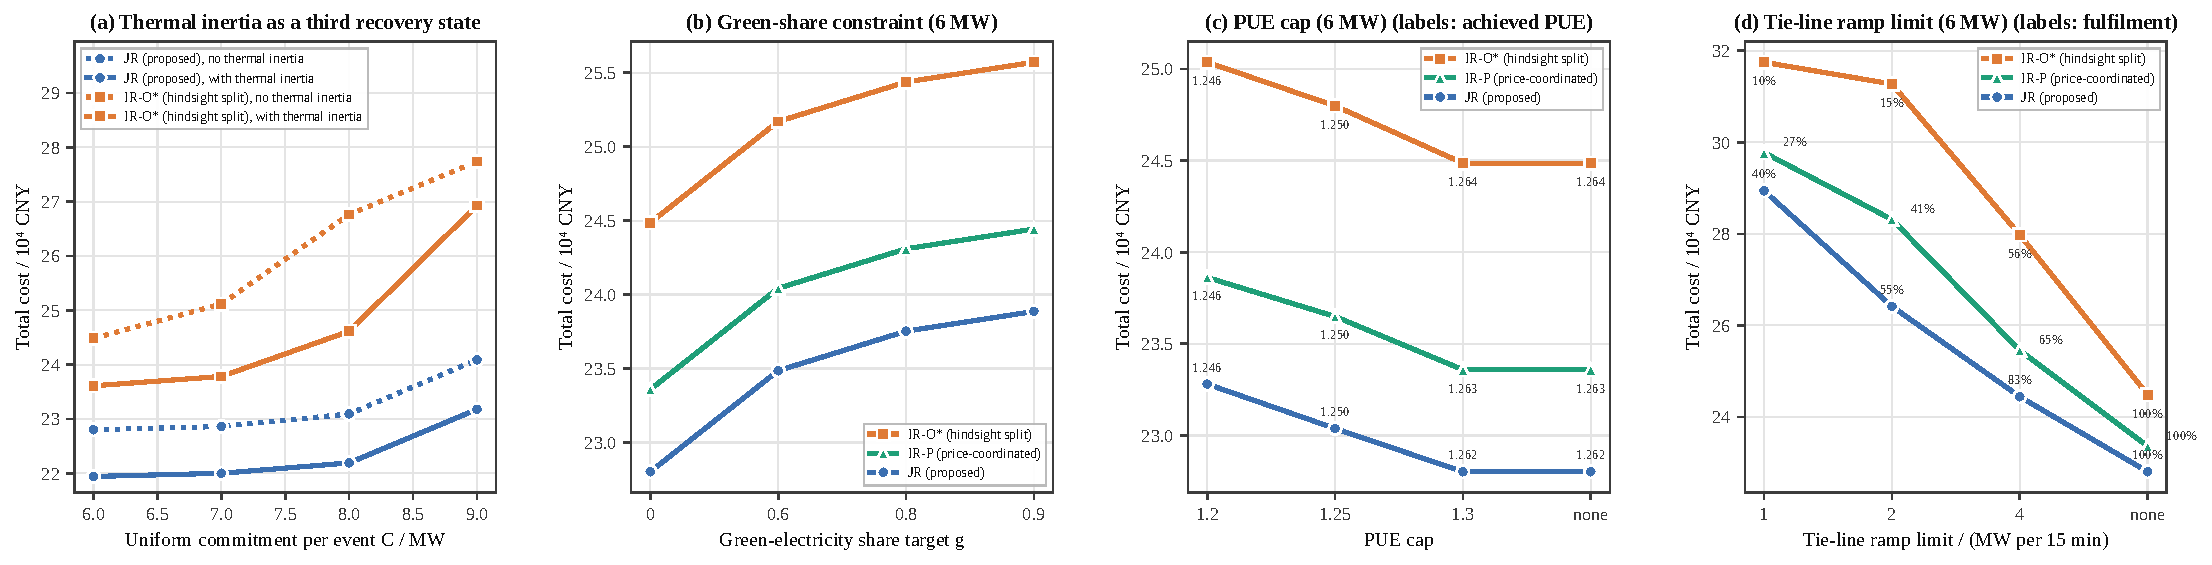
\includegraphics[width=\textwidth]{fig21_policy.pdf}
\caption{Multi-energy coupling and policy constraints ($\crb=3$, perfect information). (a) Data hall thermal inertia on
and off versus the commitment; (b) green-electricity share target; (c) PUE cap (labels: achieved PUE); (d) tie-line
ramp limit (labels: fulfilment).}
\label{fig:policy}
\end{figure*}

\figref{fig:policy} adds multi-energy coupling and policy constraints. Data hall thermal inertia acts as a third
recovery state: allowing the hall to float between $-2$ and $+3$~K around the set-point, all strategies use the full
3.0~K and save 0.86--0.88$\times10^4$~CNY per day (JR: 22.80 to 21.94), and in closed loop on 26 days JR-D saves 3.8\%
and IR-P 4.3\%. Thermal inertia is another free and fast storage that the facility side can use under independent
recovery too: at 8~MW the fulfilment of IR-P rises from 92.9\% to 99.4\%, level with JR (99.5\%). The advantage of joint
recovery remains but shrinks ($-2.6\%$ under perfect information at 8~MW, $-2.2\%$ in closed loop with
$p=1.5\times10^{-7}$), because more storage-side flexibility partly substitutes for joint recovery, as with large
batteries in \secref{sec:res-capacity}. Green-electricity targets of 60/80/90\% raise the daily cost of all strategies
by 0.68/0.95/1.08$\times10^4$~CNY with differences below 10~CNY between them, \ie\ in this accounting a green share acts
like a uniform surcharge on grid and gas electricity and does not change the ranking. Without a PUE cap, the PUE on the
DR day is 1.262--1.264; a cap of 1.25 is met by all strategies at an extra cost of 0.24 (JR) to 0.31 (IR-O*)
$\times10^4$~CNY by more absorption cooling, night-time TES charging and catch-up in cooler hours, whereas a cap of
1.20 is infeasible on this hot day (the minimum is 1.246, at 0.48--0.55$\times10^4$~CNY). Tie-line ramp limits of 4/2/1~MW
per 15~min directly restrict a fast load drop at the start of an event: the fulfilment of JR falls to
82.9/54.6/40.2\%, that of the benchmarks more (IR-P 64.9/41.2/27.2\%), and JR is 4.0/6.7/2.8\% cheaper than IR-P.
Without the limit, the largest step change of JR is a drop of 8.8~MW and a rise of 12.4~MW; since the Jiangsu rules judge
validity by the hourly mean, such ramp requirements would have to be designed together with the validity rule.

\subsubsection{Tariff shapes, seasons and climates}
\label{sec:sens-gen}

Five TOU shapes with the same daily mean are compared on 20 operating days (\figref{fig:gen}(a), \tabref{tab:tariff}).
The advantage of joint recovery is almost independent of the tariff shape: the cost reduction against IR-P is
2.1--2.9\% ($p\le4\times10^{-6}$), and the fulfilment of JR at 8~MW under perfect information is 99.5\% for every shape.
It is smallest under a flat tariff, where it matters less to which hours catch-up and recharging are moved.

\begin{table}[!t]
\caption{Tariff shapes (same daily mean): mean cost on 20 days ($10^4$~CNY) and fulfilment at 8~MW.}
\label{tab:tariff}
\centering\footnotesize
\setlength{\tabcolsep}{2.6pt}
\begin{tabular}{@{}lccc@{}}
\toprule
Tariff shape & \makecell{IR-O* / IR-P / JR-D} & \makecell{JR-D vs IR-P\\(paired)} & \makecell{8-MW fulfilment\\IR-O* / IR-P / JR}\\
\midrule
Jiangsu TOU (base) & 24.21 / 23.09 / 22.43 & $-2.86\%$ & 74.5 / 92.9 / 99.5\%\\
Flat & 27.94 / 27.08 / 26.51 & $-2.11\%$ & 74.5 / 93.0 / 99.5\%\\
Two-tier (peak 8--22~h) & 24.94 / 24.03 / 23.40 & $-2.61\%$ & 75.5 / 93.0 / 99.5\%\\
Critical peak (19--21~h) & 24.13 / 22.96 / 22.30 & $-2.85\%$ & 76.4 / 92.9 / 99.5\%\\
Duck curve & 25.20 / 24.22 / 23.53 & $-2.84\%$ & 69.3 / 92.9 / 99.5\%\\
\bottomrule
\end{tabular}
\end{table}

\begin{figure*}[!t]
\centering
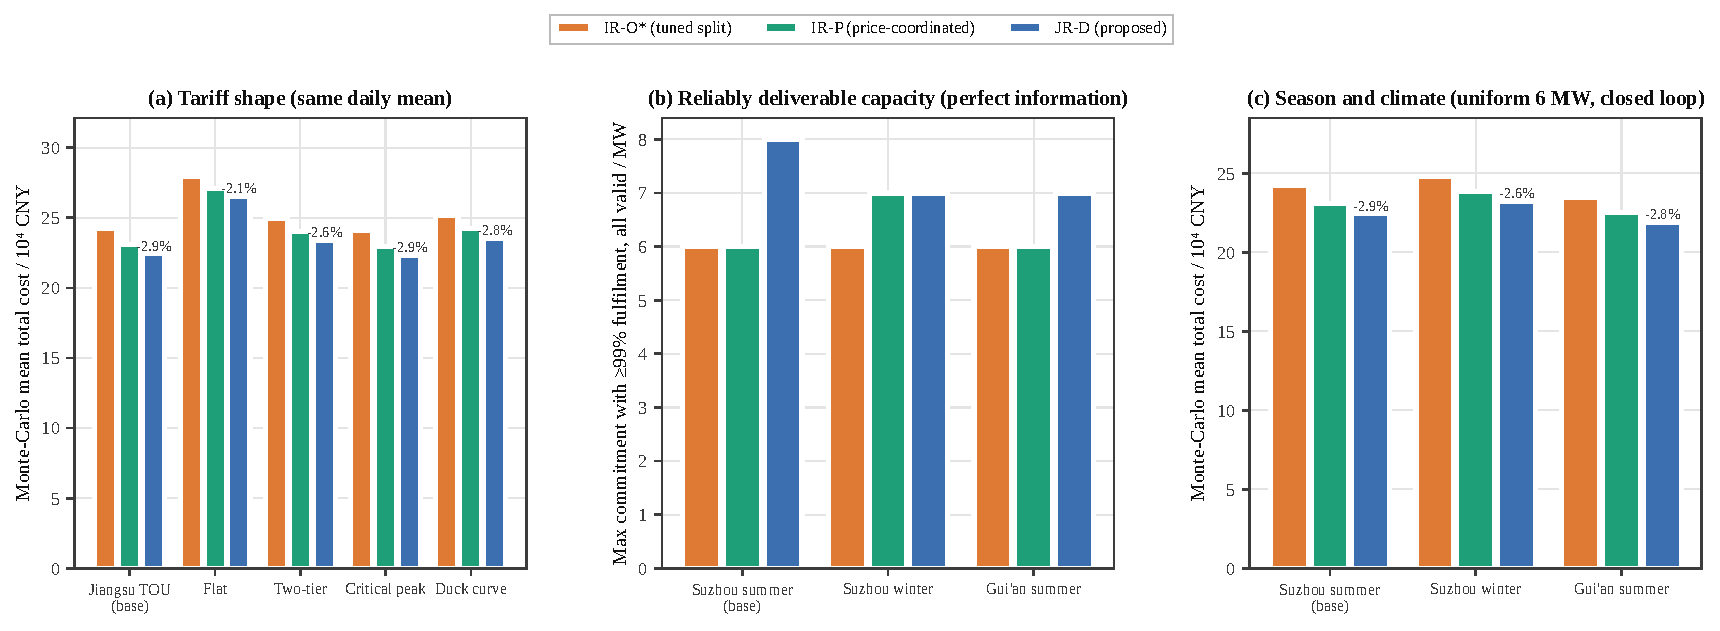
\includegraphics[width=0.98\textwidth]{fig20_generalization.pdf}
\caption{Generalisation. (a) TOU tariff shapes with the same daily mean (labels: JR-D relative to the stronger
benchmark); (b) reliably deliverable capacity under perfect information and (c) closed-loop mean cost for three climates.}
\label{fig:gen}
\end{figure*}

\begin{table}[!t]
\caption{Seasons and climates (same computing traces, Jiangsu rules and tariff).}
\label{tab:climate}
\centering\footnotesize
\setlength{\tabcolsep}{2.4pt}
\begin{tabular}{@{}lcccccc@{}}
\toprule
Case & \makecell{$\Pcap$\\(MW)} & \makecell{Mean\\COP} & \makecell{PV\\(MWh/d)} & \makecell{Reliable cap.\\IR-O*/IR-P/JR\\(MW)} & \makecell{All valid\\IR-O*/IR-P/\\JR-D} & \makecell{JR-D\\vs IR-P}\\
\midrule
\makecell[l]{Suzhou\\summer} & 16.03 & 5.13 & 38.9 & 6 / 6 / \textbf{8} & 90 / 95 / \textbf{100\%} & $-2.86\%$\\
\makecell[l]{Suzhou\\winter} & 15.51 & 7.00 & 26.0 & 6 / 7 / \textbf{7} & 95 / 95 / \textbf{100\%} & $-2.61\%$\\
\makecell[l]{Gui'an\\summer} & 15.67 & 5.77 & 44.9 & 6 / 6 / \textbf{7} & 95 / 95 / \textbf{100\%} & $-2.80\%$\\
\bottomrule
\multicolumn{7}{@{}p{0.97\columnwidth}@{}}{\scriptsize Reliable capacity under perfect information ($\ge$99\% fulfilment, all events valid); closed loop on 20 days at 6~MW, paired $p=4\times10^{-6}$ in all cases.}
\end{tabular}
\end{table}

Three climates use the same computing traces, Jiangsu rules and tariff: summer in Suzhou (base, maximum 38.3~$^\circ$C),
winter in Suzhou (10 January 2025, minimum $-3.0~^\circ$C) and summer in Gui'an (26 July 2024, maximum 31.7~$^\circ$C), a
national computing hub (\tabref{tab:climate}). In all three, JR-D keeps every event valid on every day and costs about
2.6--2.9\% less than IR-P. In winter and in the cooler climate the cooling load is lower and the COP higher, so less
cooling-related electricity can be shifted and the reliable capacity of JR drops to 7~MW; in winter IR-P also reaches
7~MW. The value of joint recovery thus follows the scarcity of the recovery channel, as Theorem~\ref{thm:closed}
predicts, and is largest in the evening peak of hot summer days. The coincidence of the drivers explains why that peak is
tight (\figref{fig:drivers}): in normal operation the storage discharges in the peak-price hours, which lowers the
17:00--22:00 baseline to about 9.6~MW, and PV has vanished while the price is still high, so reductions must rely more
on deferring computing and extra storage discharge, and the subsequent recovery need is larger.

\subsection{Job-level validation and extensions}
\label{sec:res-ext}

\subsubsection{Job-level validation of the fluid workload model}
\label{sec:res-job}

All results so far rely on the fluid model, in which backlog can be worked off on any idle GPU with any parallelism. To
test this assumption, every closed-loop run is replayed by a job-level executor and settled again. Jobs are sampled from
the joint gang-size--run-time distribution of the traces; every 15~min the deviation of each class from its nominal load
in the fluid plan becomes a target number of busy GPUs, and jobs are scheduled by slack (jobs whose slack is shorter than
one step must run) and back-filled towards the class and total targets. Jobs are rigid: they run as whole gangs at
nominal speed and cannot be accelerated. A pause costs a checkpoint before it (base: 1~min, during which the GPUs still
draw power) and a restart after it (base: 5~min of powered, unproductive time), with a minimum pause of 15~min; these
values follow asynchronous and in-memory checkpointing~\cite{wan2025,wang2023gemini,hu2024acme}. Deviations of the busy
GPUs from the fluid plan are converted into IT power, the cooling deviation is taken up by the electric chillers, and the
storage and gas engine follow the fluid plan.

On the PAI case day (\figref{fig:jobsim}(a)), the fluid plan of JR-D schedules large catch-up after each event (about
$+3$~MW of IT power after E1 and $+3$ to $+5$~MW after E3), mainly of long jobs. Rigid jobs cannot do this: 11,543
GPU$\cdot$h of the planned catch-up cannot be executed, the slack of the jobs is exhausted before E3, and E3 achieves
only 3.7~MW (below the validity threshold of 4.8~MW), so that E3 becomes invalid and the cost rises from 22.84 to
$30.98\times10^4$~CNY (+36\%). The other five strategies also lose at least one event at job level. With the rigid-job
bound \eqref{eq:rigid}, the plan of JR-D changes: E1 mainly pauses medium jobs, E2 medium and long jobs, and E3 all long
jobs, whose backlog (about 3,900~GPU$\cdot$h) is carried into the next day and worked off after their nominal ends
(\figref{fig:jobsim}(b)). The planned cost rises to $25.15\times10^4$~CNY (+10\%), because catch-up in the gaps is no
longer available, and the job-level cost is $26.52\times10^4$~CNY (+5.4\%, mostly pause and restart overheads) with all
three events valid, a tracking error of the grid import of 0.22~MW and only 397~GPU$\cdot$h of planned catch-up left
unexecuted.

\begin{table}[!t]
\caption{Job-level execution on 52 operating days.}
\label{tab:jobsim}
\centering\footnotesize
\setlength{\tabcolsep}{2.5pt}
\begin{tabular}{@{}lccc@{}}
\toprule
\makecell[l]{Load $\cdot$ recovery\\model of the plan} & \makecell{All events valid:\\JR-D / best IR} & \makecell{Job-level cost of JR-D\\vs best IR} & \makecell{JR-D job-level\\vs fluid cost}\\
\midrule
PAI $\cdot$ fluid & 5.8\% / 0\% & $-4.7\%$ (IR-P, 52/52) & +34.9\%\\
PAI $\cdot$ rigid & 86.5\% / 46--60\% & $-3.0\%$ (IR-P, 50/52) & +6.9\%\\
Acme $\cdot$ fluid & 65\% / 33--35\% & $-7.8\%$ (IR-P, 50/52) & +30.7\%\\
Acme $\cdot$ rigid & 98\% / 75--87\% & $-5.0\%$ (IR-O*, 51/52) & --\\
\bottomrule
\multicolumn{4}{@{}p{0.97\columnwidth}@{}}{\scriptsize Best IR: IR-O* and IR-P; numbers of days on which JR-D is cheaper in brackets; paired $p\le10^{-9}$.}
\end{tabular}
\end{table}

\begin{figure*}[!t]
\centering
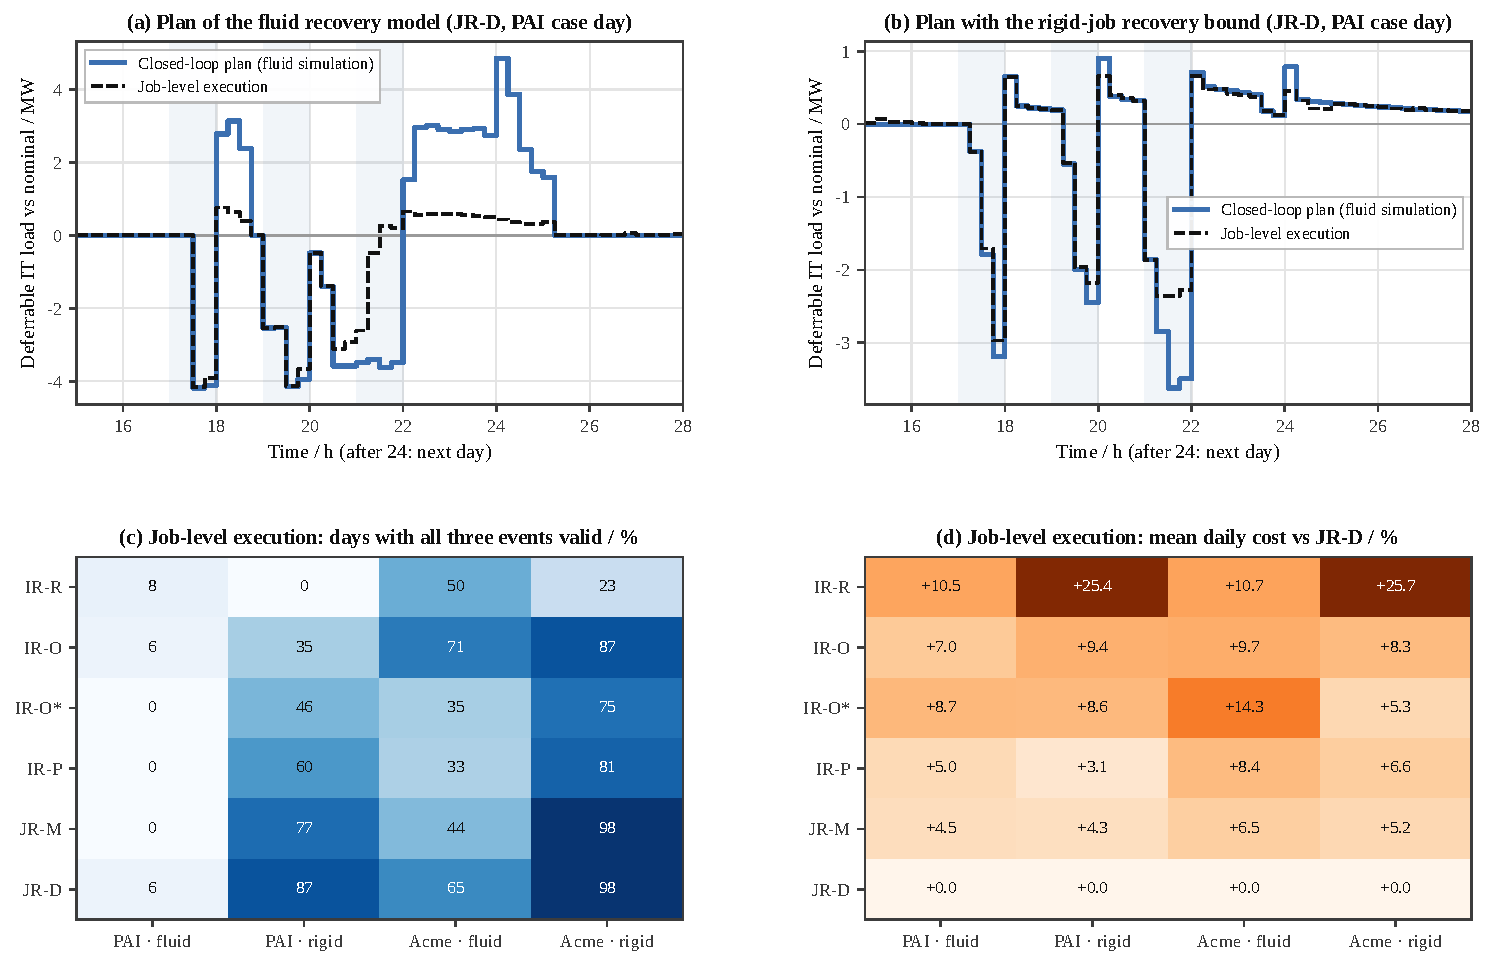
\includegraphics[width=0.90\textwidth]{fig22_jobsim.pdf}
\caption{Job-level validation. (a)(b) Closed-loop plan and job-level execution of JR-D on the PAI case day (deferrable
IT load relative to nominal) with (a) the fluid recovery model and (b) the rigid-job recovery bound; (c)(d) share of the
52 days with all events valid and mean daily cost relative to JR-D at job level.}
\label{fig:jobsim}
\end{figure*}

On the 52 days (\tabref{tab:jobsim}, \figref{fig:jobsim}(c)(d)), the fluid model proves too optimistic for rigid long
jobs: plans made with it fail at job level almost every day with the PAI load (no strategy keeps all events valid on
more than 8\% of the days) and underestimate the cost by 11--38\%; with the Acme load, where long jobs carry 80\% of the
work, all events remain valid on only 33--71\% of the days. The rigid-job bound makes the plans executable: JR-D keeps
all events valid on 98\% of the days with the Acme load and on 86.5\% (instead of 5.8\%) with the PAI load, with a
tracking error of about 0.2--0.3~MW, and the job-level cost of the same strategy is 12--16\% lower when planned with the
rigid model (JR-D: 22.13 against $25.12\times10^4$~CNY per day for Acme, 26.13 against 30.39 for PAI). The advantage of
joint recovery persists at job level: it widens to 4.7--7.8\% with fluid plans and is 5.0\% (Acme) and 3.0\% (PAI) with
rigid plans, not less than the 2.9--3.1\% of the fluid evaluation. The rigid jobs restrict catch-up in the gaps, so more
of the channel can only recharge storage, at efficiency $\eta$; independent recovery relies on catch-up in the gaps to
free the virtual storage and suffers more, whereas joint recovery carries the long-job backlog beyond the last event. In
the rigid variant the fluid accounting by arrival batches reports overdue work that does not exist (46--638
GPU$\cdot$h$\cdot$h for Acme), because the tails of finishing delayed jobs supply catch-up that the first-order bound
$B/\tau_c$ omits; the job-level results, with zero overdue work, are therefore authoritative for this variant. On its
own, the LLM-era Acme load leaves the conclusions of the fluid model unchanged: JR-D is 3.1\% cheaper than IR-P (52/52
days, $p=3.5\times10^{-10}$), similar to the 2.9\% with PAI, with all events valid on 100\% against 98\% of the days.

\begin{figure*}[!t]
\centering
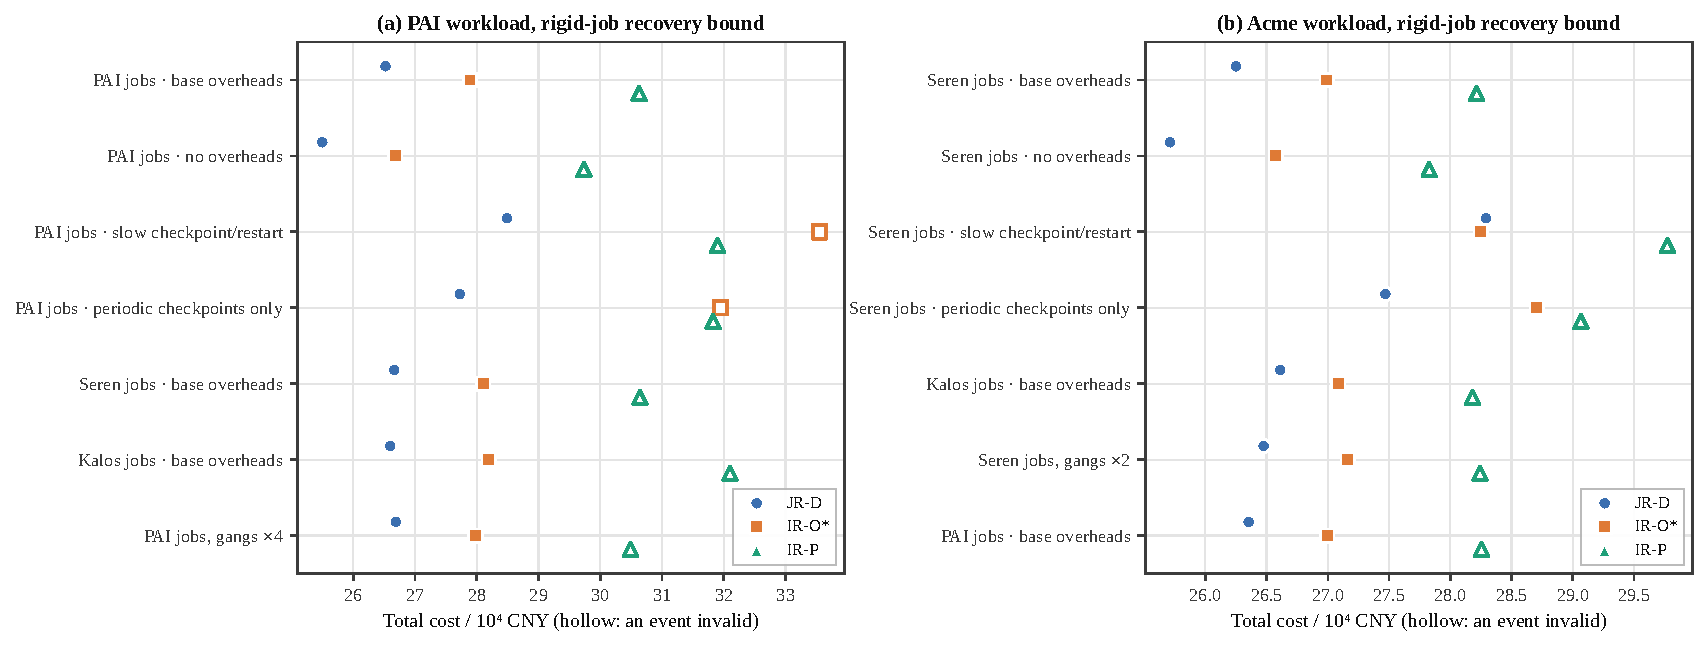
\includegraphics[width=0.90\textwidth]{fig23_jobmix.pdf}
\caption{Job-level total cost on the case day for different job mixes and pause overheads (rigid-job recovery bound;
hollow markers: at least one event invalid).}
\label{fig:jobmix}
\end{figure*}

The job mix and overheads are varied on the case day in \figref{fig:jobmix}: jobs from Seren or Kalos (pre-training
jobs with 512--1,024 GPUs), gang sizes scaled by 2 or 4, and no, base, slow (10-min checkpoint, 15-min restart, 30-min
minimum pause) or periodic-only checkpointing (every 30~min, losing the progress since the last checkpoint). Plans made
with the rigid model are executable in all settings: in all 14 load--job combinations JR-D keeps all three events valid
and is the cheapest in 13; the exception is the Acme load with slow checkpoint and restart, where IR-O* is 0.15\% cheaper
with all events valid as well. With the PAI load the job-level cost exceeds the fluid evaluation by 1.4\% without
overheads, 5.5\% with base overheads and 13\% with slow ones. The strongest benchmarks are more sensitive to overheads:
with the PAI load and slow checkpointing IR-O* keeps only one event valid (two with periodic checkpointing only), and IR-P
loses at least one event in every setting (two with Kalos jobs); with base overheads JR-D is 4.9\% (PAI) and 2.7\%
(Acme) cheaper than IR-O* at job level. With base overheads a day sees 650--4,100 pauses (more with small jobs), about
1,100--1,400~GPU$\cdot$h of restarts and 220--300~GPU$\cdot$h of lost checkpoint progress, together about 1.3--1.6~MWh,
which raises the daily cost of JR-D by 2--4\%; slow checkpointing roughly triples these overheads. Gang granularity
matters little: even when the largest paused job draws 0.7--1.2~MW, the cost of JR-D changes by only 0.3--1.4\%, since
the executor back-fills with small jobs and other classes absorb the granularity error. All pauses at the start of an
event complete within the same minute, so the deferrable IT power steps by about 3--4~MW within 1~min; if the grid
limits ramps, the pauses can be staggered over a few minutes or the IT ramp limit of \secref{sec:computing} can be
imposed. Power swings of synchronous training at the second and iteration scale~\cite{choukse2025} are outside the 15-min
scheduling considered here.

\subsubsection{Pause overheads and multi-level power capping}
\label{sec:ext-overhead}

The fluid model is extended by the pause overhead $o_c$ of \eqref{eq:backlog} (base: 6~min per newly paused GPU for a
1-min asynchronous checkpoint and a 5-min restart; slow: 25~min for synchronous checkpoints and slow restarts of large
models) and by power capping with one level (power $-30\%$, throughput $-12\%$) or three levels ($-15/-30/-45\%$ power
for $-3/-12/-30\%$ throughput), with uniform 6~MW, re-tuned benchmarks and 26 days (\tabref{tab:overhead},
\figref{fig:ext}(a)).

\begin{table*}[!t]
\caption{Pause overheads and multi-level power capping (26 days, uniform 6~MW).}
\label{tab:overhead}
\centering\footnotesize
\setlength{\tabcolsep}{6pt}
\begin{tabular}{@{}lcccc@{}}
\toprule
Setting & \makecell{JR-D cost\\($10^4$~CNY)} & \makecell{JR-D vs\\IR-P} & \makecell{All valid\\JR-D/IR-P/IR-O*} & \makecell{Overhead (GPU$\cdot$h)\\JR-D/IR-P/IR-O*}\\
\midrule
Base (fluid) & 22.50 & $-2.8\%$ (25/26) & 100/96/92\% & --\\
Overhead 6~min & 23.20 & $-2.6\%$ (25/26) & 96/88/62\% & 1,465/1,761/2,919\\
Overhead 25~min & 24.10 & $-2.3\%$ (24/26) & 100/81/27\% & 3,869/4,686/5,624\\
One capping level & 21.87 & $-4.8\%$ (26/26) & 100/62/65\% & --\\
Three capping levels & 21.83 & $-4.5\%$ (26/26) & 100/65/65\% & --\\
Three levels + 6~min & 22.55 & $-2.6\%$ (22/26) & 96/58/38\% & 1,169/1,111/244\\
\bottomrule
\multicolumn{5}{@{}l@{}}{\scriptsize Paired Wilcoxon $p<4\times10^{-4}$ in all settings.}
\end{tabular}
\end{table*}

Pause overheads raise the cost by 3.1\% (6~min) and 7.1\% (25~min), the same order as in the job-level simulation
(2--4\%). JR-D remains the cheapest, with its advantage over IR-P narrowing from 2.8\% to 2.3\%, but the reliability of
the independent benchmarks falls faster: IR-O* keeps all events valid on only 62\% and 27\% of the days. Since the
overhead counts newly paused GPUs, the static split of IR-O*, which pauses and resumes repeatedly between events, incurs
the largest overhead, whereas JR-D defers long jobs continuously and incurs the smallest (half that of IR-O* at 6~min).
Power capping makes every strategy cheaper and widens the advantage of joint recovery: the cost of JR-D falls by 2.8\%
and its advantage over IR-P grows to 4.5--4.8\% (26/26 days). The throughput loss of capping becomes additional
backlog; IR-P keeps all events valid on only 62--65\% of the days instead of 96\%, while JR-D stays at 100\%, consistent
with joint recovery scheduling the backlog left by capping together with the storage deficit across events. Three
levels are only 0.2\% cheaper than one, so a single level of $-30\%$ power for $-12\%$ throughput is nearly sufficient.
With both capping and overheads the two effects largely cancel: JR-D costs $22.55\times10^4$~CNY, close to the base, and
is still 2.6\% cheaper than IR-P (22/26 days); IR-O* then caps more and pauses less (244~GPU$\cdot$h of overhead) but
keeps all events valid on only 38\% of the days.

\subsubsection{Green-power direct supply with offshore wind}
\label{sec:ext-wind}

Offshore wind from the Rudong site is connected behind the meter without grid export under the green-power
direct-connection policy~\cite{ndrc2025green}, which requires the self-consumed share to be at least 60\% of the usable
generation and at least 30\% (35\% before 2030) of the user's consumption. The connection limit stays at 16.0~MW, the
day-ahead wind forecast has an error of 15\% of the capacity (root mean square), and each operating day re-solves the
day-ahead commitment and the IR-P price with its own forecast (\tabref{tab:wind}, \figref{fig:wind}). Without DR, the
renewable share of consumption averages 25.6/40.0/58.4/71.9\% at 5/10/20/40~MW of wind, and the self-consumed share stays
at 100\% up to 10~MW and falls to 89.1\% at 20~MW and 65.5\% at 40~MW. The policy evaluates both shares annually; on
average about 7~MW of wind meets the 30\% share and 40~MW still meets the 60\% self-use, while on a daily basis both
are met on most days at 20~MW (94\%; 91\% with the 35\% threshold), so a wind capacity of about 1.25 times the connection
limit matches the policy best.

\begin{table*}[!t]
\caption{DR with behind-the-meter offshore wind (26 operating days).}
\label{tab:wind}
\centering\footnotesize
\setlength{\tabcolsep}{6pt}
\begin{tabular}{@{}ccccccc@{}}
\toprule
\makecell{Wind\\(MW)} & \makecell{Wind\\(MWh/d)} & \makecell{Commitment sum\\(MW, declared)} & \makecell{JR-D DR revenue\\($10^4$~CNY/d)} & \makecell{JR-D cost\\($10^4$~CNY)} & \makecell{JR-D vs\\IR-P} & \makecell{All valid\\JR-D/IR-P/IR-O*}\\
\midrule
0 & 0 & 17.7 (100\%) & 6.21 & 22.46 & $-2.5\%$ & 100/96/96\%\\
5 & 50 & 13.4 (96\%) & 4.41 & 18.99 & $-6.6\%$ & 92/58/92\%\\
10 & 100 & 7.8 (92\%) & 2.36 & 16.21 & $-6.6\%$ & 77/46/58\%\\
20 & 199 & 6.6 (100\%) & 2.08 & 10.77 & $-5.9\%$ & 85/73/65\%\\
\bottomrule
\multicolumn{7}{@{}l@{}}{\scriptsize Paired differences: 25/26, 24/26, 24/26 and 21/26 days cheaper; $p$ = $9\times10^{-8}$, $1\times10^{-6}$, $3\times10^{-6}$ and 0.002.}
\end{tabular}
\end{table*}

\begin{figure*}[!t]
\centering
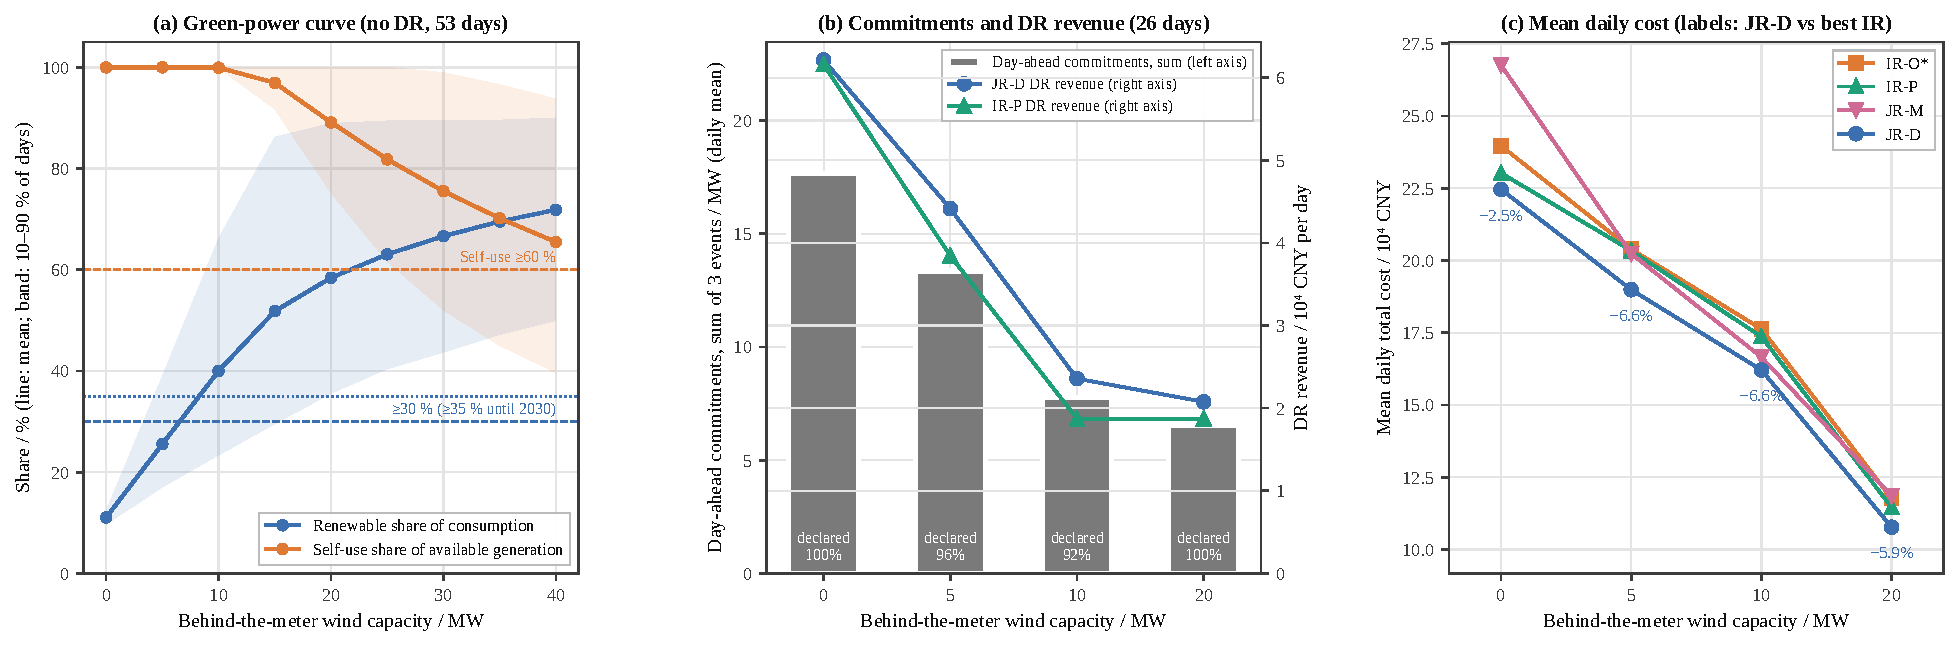
\includegraphics[width=0.98\textwidth]{fig26_wind.pdf}
\caption{Green-power direct supply with offshore wind. (a) Renewable share of consumption and self-used share of the
available generation without DR (lines: means; bands: 10--90\% of the days) with the policy thresholds; (b) sum of the
day-ahead commitments (bars; share of declared events inside) and DR revenue; (c) mean daily cost (labels: JR-D
relative to the strongest independent benchmark).}
\label{fig:wind}
\end{figure*}

The meter-based baseline makes the deliverable commitments fall quickly with the wind capacity. The baseline is taken
from the meter data of the reference days and thus inherits their wind; once the wind of the operating day deviates from
that average, the metered ``reduction'' deviates as well even if the load does not. The total commitment falls from 17.7
to 6.6~MW at 20~MW of wind ($-63\%$), the DR revenue of JR-D drops to one third, and on days with little forecast wind the
day-ahead model declares some events with zero commitment (8\% of the events at 10~MW). The saved electricity cost far
exceeds the lost DR revenue: the daily cost of JR-D falls from 22.5 to $10.8\times10^4$~CNY at 20~MW. The advantage of
joint recovery widens with wind, to 5.9--6.6\% against IR-P (2.5\% without wind), because forecast errors shift the net
load during the events and reduce validity for all strategies, but less for joint recovery, which keeps more margin for
corrections by planning backlog and storage across events (all events valid on 77--92\% of the days against 46--73\%
for IR-P). The differences come from days with weak and mispredicted wind, whereas on the windy case day (122 and
244~MWh at 10 and 20~MW) commitments are small and easy to meet and the strategies differ by less than 1\%. Measuring
the baseline at the grid meter thus counts the fluctuations of behind-the-meter wind as response or counter-response
(see~\cite{chao2011} for baseline choice in general); metering the wind separately and settling on the load net of wind
would preserve the flexibility of the data center, which needs clarification at the policy level.

\subsubsection{Winter waste-heat recovery}
\label{sec:ext-heat}

In winter, a water-source heat pump (3~MW$_{\mathrm{el}}$, COP 3.5) lifts the waste heat of the chilled-water return to
a nearby heat network through a hot-water tank \eqref{eq:heat}, with the gas boiler as backup. The case day is the cold
day of 10 January 2025 (daily mean 0.4~$^\circ$C), the heat demand is about 5.3~MW$_{\mathrm{th}}$ (127~MWh$_{\mathrm{th}}$
per day), the connection limit stays at the 15.5~MW without heating, and the 26 coldest winter days are the operating
days (\tabref{tab:heat}, \figref{fig:heat}).

\begin{table*}[!t]
\caption{Winter waste-heat recovery (26 coldest days, uniform 6~MW).}
\label{tab:heat}
\centering\footnotesize
\setlength{\tabcolsep}{6pt}
\begin{tabular}{@{}lccccc@{}}
\toprule
Setting & \makecell{JR-D cost\\($10^4$~CNY)} & \makecell{JR-D vs\\IR-P} & \makecell{All valid\\JR-D/IR-P/IR-O*} & \makecell{Waste-heat share\\JR-D / IR-P} & \makecell{Boiler (MWh)\\JR-D / IR-P}\\
\midrule
Gas boiler only & 28.25 & $-2.1\%$ (25/26) & 100/96/96\% & 0 / 0 & 138.6 / 138.6\\
Heat pump, no tank & 23.56 & $-4.4\%$ (26/26) & 100/69/96\% & 82.6 / 77.4\% & 24.1 / 31.3\\
Heat pump + 20~MWh & 23.56 & $-2.3\%$ (25/26) & 100/96/96\% & 97.1 / 91.4\% & 4.1 / 12.1\\
Heat pump + 40~MWh & 23.88 & $-1.4\%$ (25/26) & 100/96/92\% & 99.9 / 99.4\% & 0.2 / 0.8\\
\bottomrule
\multicolumn{6}{@{}l@{}}{\scriptsize Boiler heat includes the first 6~h of the next day; paired Wilcoxon $p<10^{-5}$.}
\end{tabular}
\end{table*}

\begin{figure*}[!t]
\centering
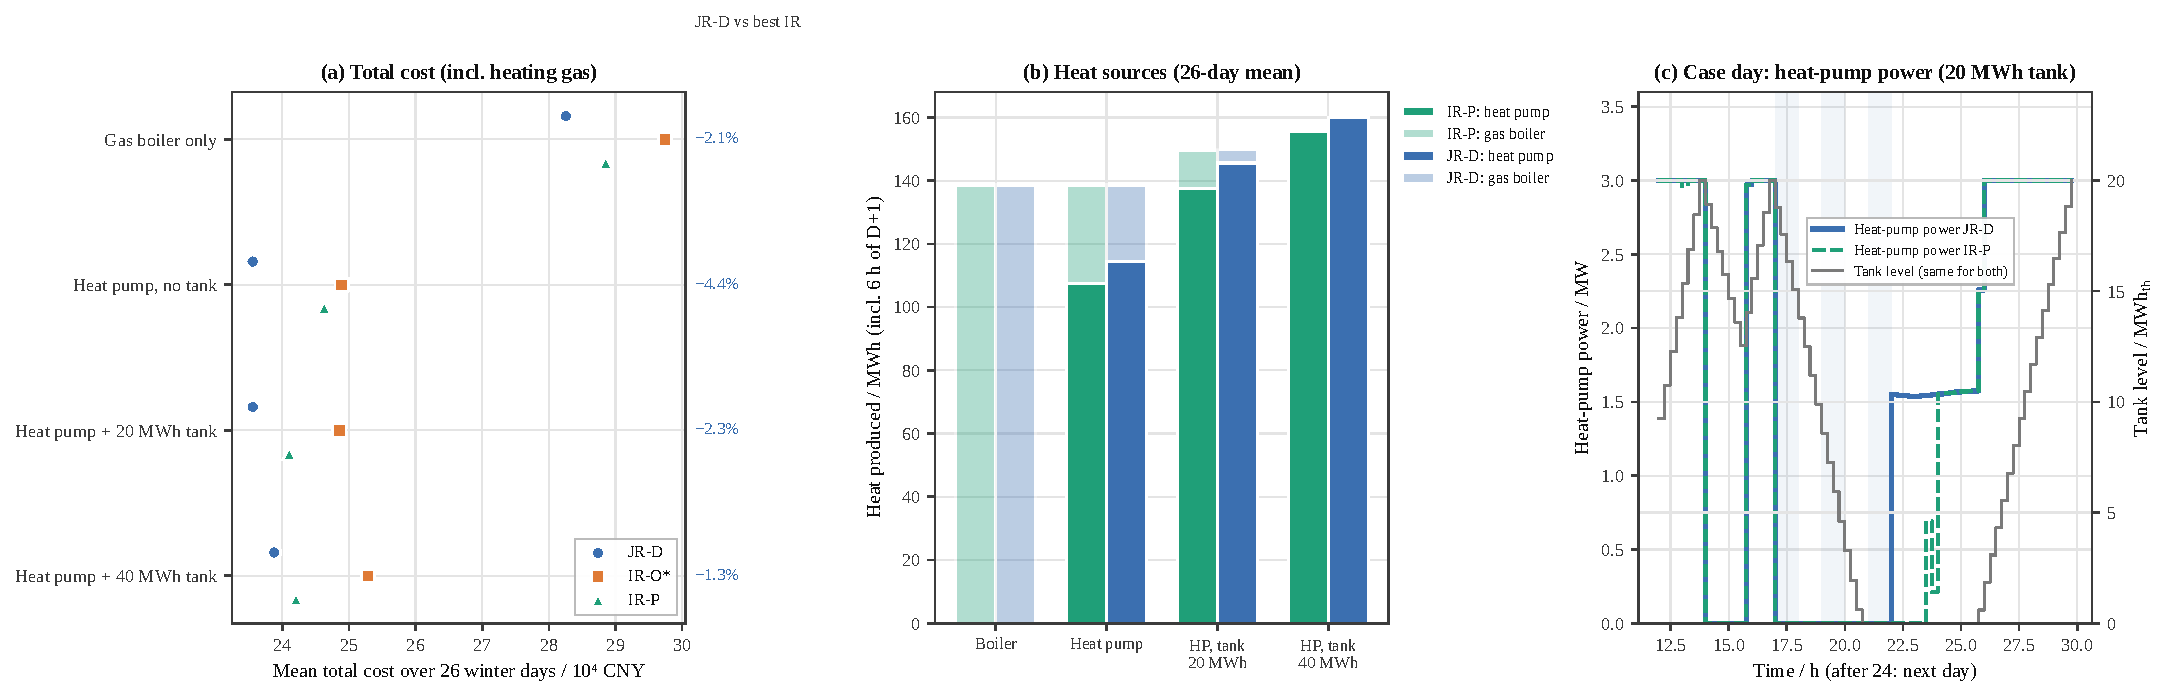
\includegraphics[width=0.98\textwidth]{fig27_heat.pdf}
\caption{Winter waste-heat recovery. (a) Mean total cost on the 26 coldest days including heating gas (right: JR-D
relative to the strongest independent benchmark); (b) heat produced by the heat pump and the gas boiler; (c) heat-pump
power and tank level on the case day with the 20-MWh tank.}
\label{fig:heat}
\end{figure*}

Waste-heat recovery pays off by itself: it lowers the daily cost by 15.5--16.6\% against boiler heating (4.4--4.7$\times
10^4$~CNY per day for JR-D) and the emissions by 16--19~t of CO$_2$ per day. Without a tank, the heat pump competes with
catch-up computing for the channel: its load is part of the baseline, so switching it off during an event counts as
reduction, but the heat demand continues and the heat pump must catch up afterwards, exactly when catch-up computing and
battery recharging need the headroom. The IT side of independent recovery takes this headroom first, so IR-P keeps all
events valid on only 69\% instead of 96\% of the days and burns more boiler gas, while joint recovery, which schedules
the heat pump together with the other states, widens its advantage to 4.4\% (26/26 days). A tank decouples heating from
the events: the heat pump stops during the events, the tank supplies the heat and is recharged afterwards. All strategies
then keep the events valid on 96--100\% of the days and the advantage returns to 2.3\%, but joint recovery recovers about
6 points more waste heat (boiler heat 4.1 against 12.1~MWh), because after E3 it gives the headroom to the heat pump
first whereas independent recovery gives it to catch-up computing (\figref{fig:heat}(c): JR-D restarts the heat pump right
after E3, IR-P about 1.5~h later, with the boiler covering the gap). A larger tank is not always better: the 40-MWh tank
already shifts all peak-period heat-pump load to the valley hours in normal operation, which lowers the baseline in the
event hours by about 0.7~MW against no tank and 0.3~MW against the 20-MWh tank (the same mechanism as for large
batteries in \secref{sec:res-capacity}); JR-D then costs 1.4\% more than with the 20-MWh tank and its advantage shrinks to
1.4\%.

\subsection{Discussion}
\label{sec:discussion}

The results support three practical implications. First, consecutive DR should be bid and settled as a whole: the
capability region of joint recovery is described by the stand-alone capabilities and one cross-event energy budget, and
declaring these virtual-battery parameters instead of one value per event lets the grid operator call more capacity with
the same reliability. Second, the main value of joint recovery lies in the reliably deliverable capacity rather than in
the operating cost at moderate commitments, and it is largest when the recovery channel is scarce: hot evening peaks,
short gaps, tight connection margins, liquid cooling, smaller batteries or a heat pump without a tank. Third, joint
recovery can be implemented without merging the IT and facility control systems, through a few plan--price exchanges per
15~min, whereas a one-shot price signal is insufficient. The settlement rules matter as well: the rebound charge, the
baseline method with storage arbitrage and behind-the-meter wind, and ramp requirements change what the data center
can deliver and should be designed together with its flexibility.

The study has limitations. The fluid workload model is optimistic for rigid gang-scheduled jobs; the rigid-job bound is
a first-order approximation, and the job-level executor is a slack-based heuristic without job dependencies, network
topology or communication overheads. The PAI trace predates LLMs and the Acme trace stems from one institution, while
frontier pre-training jobs may use thousands of GPUs. Only the call of the last event is uncertain, the scenario sets are
small and deterministic, and the ambiguity set covers only the scenario probabilities (a Wasserstein
ball~\cite{esfahani2018} would also cover unseen outcomes). The capability region is computed under perfect information.
The distributed scheme approximates the proximal term by tangent cuts and does not model communication delays, losses,
asynchronous updates or strategic behaviour. Thermal inertia, policy and waste-heat parameters take typical values, the
wind forecast errors are synthetic, the season and climate tests replace only the weather, and the system is aggregated
on one bus without distribution network constraints.

